%%%%%%%%%%%%%%%%%%%%%%%%%%%%%%%%%%%%%%%%%%%%%%%%%
%%%%%%%%%%%%%%%%%%%%%%%%%%%%%%%%%%%%%%%%%%%%%%%%%
\chapter{Results}
\label{chap:results}

The analysis of the results of the experiments is organised around four major characteristics of swarm robotics algorithms, namely efficiency, flexibility, robustness and scalability. Section~\ref{results:efficiency} addresses foraging b, while flexibility of the algorithms over different environment distributions and item type ratios is analysed in Section~\ref{results:flexibility}. Section~\ref{results:scalability} evaluates of scalability of each algorithm and robustness is analysed in Section~\ref{results:robustness}. Section~\ref{results:summary} summarizes the findings of the analysis.

\section{Foraging efficiency}
\label{results:efficiency}


Despite the fact that determining the most efficient algorithm is not a main focus of this study, this section does a brief comparison of the foraging efficiency, as defined in Section~\ref{setup:foragingefficiency}, of each algorithm. 

This is done by comparing the performance of the three algorithms over all environments and experimental parameters. A wilcoxin test, of a confidence level of 0.05, was applied to each pair of algorithms to determine if a statistically significant difference in performance of a pair of algorithms exists. If a statistically significant difference is indicated, then two one-tailed Mann-Whitney U tests were performed with a confidence level of 0.05, to determine which algorithm was more efficient on a particular experiment. TODO: explain wins and losses somehow

To determine an algorithm's foraging efficiency in comparison to all other algorithms, the wins and losses per each experiment performed for each algorithm, are summed. This statistical analysis approach has been used in \cite{helbig2013performance}.

Table~\ref{summarytable} shows the total wins and losses for each algorithm. The desert ant foraging performed better than the na\"ive algorithm. The honey bee algorithm out-performed both the na\"ive algorithm and the desert ant algorithm. The following sections analyse the swarm robotic properties of each algorithm, and explain why the foraging efficiency of the algorithms is as shown in Table\ref{summarytable}.


\begin{table}[]
\centering
\caption{Pairwise one-tailed Mann Whitney U wins and losses of $E_p$, for each algorithm, over all environments, parameter value choices }
\label{summarytable}
\begin{tabular}{@{}lll@{}}
\toprule
\textbf{Algorithms} & \textbf{Wins} & \textbf{Losses} \\ \midrule
na\"ive               & 1168          & 59042           \\
desert ant          & 42120         & 14557           \\
honey bee           & 45490         & 15179           \\ \bottomrule
\end{tabular}
\end{table}

\section{Flexibility}
\label{results:flexibility}

This section analyses the flexibility of each of the considered algorthms, in terms of the prioritized item ratio and the environment distribution types, over all experiments. Section~\ref{results:prioritizeditemratio} analyses the flexibility of each algorithm, in terms of the prioritized item ratio of the environment (refer to Section~\ref{setup:flexibility:prioritizeditemratio}). Section~\ref{results:flexibility:environmentdistribution} discusses the flexibility of each algorithm, in terms of environment distribution types, (refer to Section~\ref{setup:flexibility:environmentdistributions}).

\subsection{Flexibility in terms of prioritized item ratio}
\label{results:prioritizeditemratio}

The performance measure, $F$, measures how well swarm parameters, yielding the best efficiency for environments with a specific prioritized item ratio, generalize across environments with different prioritized item ratios. The less the foraging efficiency varies, when an algorithm that is configured with swarm parameters optimized for a specific environment ratio, is run on all other environment ratios, the smaller $F$ will be. Therefore, the smaller $F$ is, the more flexible an algorithm is considered to be. $F$ is a macro performance indicator which is run on the results of all experiments. 

Table~\ref{table:flexibility} summarizes the flexibility of each foraging algorithm in terms of environment type ratio, $F_r$. According to Table~\ref{table:flexibility}, the honey bee algorithm is the most flexible in terms of $F_r$, followed by the na\"ive algorithm, with the desert ant algorithm being the worst. 

 
% Please add the following required packages to your document preamble:
% \usepackage{booktabs}
\begin{table}[]
\centering
\caption{Flexibility in terms of prioritized item ratio, $F_r$, and flexibility in terms of environment distribution, $F_{ED}$, for each algorithm}
\label{table:flexibility}
\begin{tabular}{@{}llll@{}}
\toprule
\textbf{}         & na\"ive         & desert ant        & honey bee         \\ \midrule
\textbf{$F_r$}    & 1.18580054603 & 3.12400224646     & 0.827991739287    \\ \midrule
\textbf{$F_{ED}$} & 1.11160672365 & 0.507371308759 & 0.458295680454 
\end{tabular}
\end{table}

The honey bee algorithm is the most flexible in terms of prioritized item ratio. To understand why this is the case, one examines the mechanisms used specifically by the honey bee algorithm. In particular, the honey bee algorithm employs a division of labour mechanism that allows robots to switch from foraging prioritized items, to non-prioritized items (and vice versa). The honey bee algorithm's division of labour mechanism suggests the following hypothesis: The honey bee algorithm's superior flexibility is due to the fact that the robots can switch their item type specialization. In that way, the honey bee algorithm was able to adapt the swarm specialization ratio to more efficiently forage a given environment item type ratio.

To provide evidence for the above hypothesis, an examination of the average swarm specialization ratio over time, $\tau(t)$, for the honey bee algorithm on a uniformly distributed environment with a high ratio of prioritized items (i.e. $r = 0.75$). The initial swarm specialization ratio, $\tau(0)$ was set to 0, which means that all robots are set to forage non-prioritized items . The swarm specialization ratio over time $\tau(t)$ was averaged over 30 independent runs. The purpose behind examining the described scenario is to determine if the honey bee algorithm is able to adapt the swarm's specialization ratio (which initially can only forage non-prioritized items), to more efficiently forage the high ratio of prioritized items. The above scenario is illustrated in Figure~\ref{fig:specializationratioovertime}. 

Figure~\ref{fig:specializationratioovertime} shows that $\tau$ increased from 0 to 1 in 200 iterations, which suggests that, when the honey bee scout robots could not find any non-prioritized items, the honey bee scout robots switched their specializations to search for prioritized items instead. After 200 iterations, the specialization ratio, steadily declined from 1 to 0.73. The final swarm specialization ratio $\tau(10000)=0.73$ is nearly the same as the environment ratio, $r=0.75$, suggesting that the honey bee algorithm eventually adapted the specialization ratio to effectively forage the environment item type ratio of the given environment.

The above analysis supports the hypothesis that the honey bee algorithm's superior flexibility can be attributed to the algorithm's ability to adapt the swarm's specialization ratio, via the division of labour mechanism described in Section~\ref{natureinspired:divisionoflabour} to more efficiently forage an environment of a given environment item ratio.

The na\"ive algorithm and desert ant algorithm do not have the ability to adapt $\tau$ and are less flexible than the honey bee algorithm.

Despite the desert ant algorithm outperforming the na\"ive algorithm in efficiency, as shown in Section~\ref{results:efficiency}, the na\"ive algorithm is more flexible, according to Table~\ref{table:flexibility}. Rationally, since the na\"ive algorithm does not have high efficiency on any environment, foraging efficiency was not affected very much by any specialization ratio, unable to take advantage of any value for $r$ of $\tau_0$ and thus, will always be equally bad.

%The flexibility of the desert ant algorithm is the worst out of the considered algorithms. Table~\ref{doesnotexistyet} shows that the desert ant algorithm's performance is very dependant on the value of $\tau_0$.

\begin{figure}[!htb]
\centering
\resizebox{\textwidth}{!}{% GNUPLOT: LaTeX picture with Postscript
\begingroup
  \makeatletter
  \providecommand\color[2][]{%
    \GenericError{(gnuplot) \space\space\space\@spaces}{%
      Package color not loaded in conjunction with
      terminal option `colourtext'%
    }{See the gnuplot documentation for explanation.%
    }{Either use 'blacktext' in gnuplot or load the package
      color.sty in LaTeX.}%
    \renewcommand\color[2][]{}%
  }%
  \providecommand\includegraphics[2][]{%
    \GenericError{(gnuplot) \space\space\space\@spaces}{%
      Package graphicx or graphics not loaded%
    }{See the gnuplot documentation for explanation.%
    }{The gnuplot epslatex terminal needs graphicx.sty or graphics.sty.}%
    \renewcommand\includegraphics[2][]{}%
  }%
  \providecommand\rotatebox[2]{#2}%
  \@ifundefined{ifGPcolor}{%
    \newif\ifGPcolor
    \GPcolorfalse
  }{}%
  \@ifundefined{ifGPblacktext}{%
    \newif\ifGPblacktext
    \GPblacktexttrue
  }{}%
  % define a \g@addto@macro without @ in the name:
  \let\gplgaddtomacro\g@addto@macro
  % define empty templates for all commands taking text:
  \gdef\gplbacktext{}%
  \gdef\gplfronttext{}%
  \makeatother
  \ifGPblacktext
    % no textcolor at all
    \def\colorrgb#1{}%
    \def\colorgray#1{}%
  \else
    % gray or color?
    \ifGPcolor
      \def\colorrgb#1{\color[rgb]{#1}}%
      \def\colorgray#1{\color[gray]{#1}}%
      \expandafter\def\csname LTw\endcsname{\color{white}}%
      \expandafter\def\csname LTb\endcsname{\color{black}}%
      \expandafter\def\csname LTa\endcsname{\color{black}}%
      \expandafter\def\csname LT0\endcsname{\color[rgb]{1,0,0}}%
      \expandafter\def\csname LT1\endcsname{\color[rgb]{0,1,0}}%
      \expandafter\def\csname LT2\endcsname{\color[rgb]{0,0,1}}%
      \expandafter\def\csname LT3\endcsname{\color[rgb]{1,0,1}}%
      \expandafter\def\csname LT4\endcsname{\color[rgb]{0,1,1}}%
      \expandafter\def\csname LT5\endcsname{\color[rgb]{1,1,0}}%
      \expandafter\def\csname LT6\endcsname{\color[rgb]{0,0,0}}%
      \expandafter\def\csname LT7\endcsname{\color[rgb]{1,0.3,0}}%
      \expandafter\def\csname LT8\endcsname{\color[rgb]{0.5,0.5,0.5}}%
    \else
      % gray
      \def\colorrgb#1{\color{black}}%
      \def\colorgray#1{\color[gray]{#1}}%
      \expandafter\def\csname LTw\endcsname{\color{white}}%
      \expandafter\def\csname LTb\endcsname{\color{black}}%
      \expandafter\def\csname LTa\endcsname{\color{black}}%
      \expandafter\def\csname LT0\endcsname{\color{black}}%
      \expandafter\def\csname LT1\endcsname{\color{black}}%
      \expandafter\def\csname LT2\endcsname{\color{black}}%
      \expandafter\def\csname LT3\endcsname{\color{black}}%
      \expandafter\def\csname LT4\endcsname{\color{black}}%
      \expandafter\def\csname LT5\endcsname{\color{black}}%
      \expandafter\def\csname LT6\endcsname{\color{black}}%
      \expandafter\def\csname LT7\endcsname{\color{black}}%
      \expandafter\def\csname LT8\endcsname{\color{black}}%
    \fi
  \fi
    \setlength{\unitlength}{0.0500bp}%
    \ifx\gptboxheight\undefined%
      \newlength{\gptboxheight}%
      \newlength{\gptboxwidth}%
      \newsavebox{\gptboxtext}%
    \fi%
    \setlength{\fboxrule}{0.5pt}%
    \setlength{\fboxsep}{1pt}%
\begin{picture}(7200.00,5040.00)%
    \gplgaddtomacro\gplbacktext{%
      \csname LTb\endcsname%
      \put(740,640){\makebox(0,0)[r]{\strut{}$0$}}%
      \put(740,1056){\makebox(0,0)[r]{\strut{}$0.1$}}%
      \put(740,1472){\makebox(0,0)[r]{\strut{}$0.2$}}%
      \put(740,1888){\makebox(0,0)[r]{\strut{}$0.3$}}%
      \put(740,2304){\makebox(0,0)[r]{\strut{}$0.4$}}%
      \put(740,2720){\makebox(0,0)[r]{\strut{}$0.5$}}%
      \put(740,3135){\makebox(0,0)[r]{\strut{}$0.6$}}%
      \put(740,3551){\makebox(0,0)[r]{\strut{}$0.7$}}%
      \put(740,3967){\makebox(0,0)[r]{\strut{}$0.8$}}%
      \put(740,4383){\makebox(0,0)[r]{\strut{}$0.9$}}%
      \put(740,4799){\makebox(0,0)[r]{\strut{}$1$}}%
      \put(860,440){\makebox(0,0){\strut{}$0$}}%
      \put(2056,440){\makebox(0,0){\strut{}$2000$}}%
      \put(3252,440){\makebox(0,0){\strut{}$4000$}}%
      \put(4447,440){\makebox(0,0){\strut{}$6000$}}%
      \put(5643,440){\makebox(0,0){\strut{}$8000$}}%
      \put(6839,440){\makebox(0,0){\strut{}$10000$}}%
    }%
    \gplgaddtomacro\gplfronttext{%
      \csname LTb\endcsname%
      \put(160,2719){\rotatebox{-270}{\makebox(0,0){\strut{}$\tau(t)$}}}%
      \put(3849,140){\makebox(0,0){\strut{}timesteps ($t$)}}%
      \put(5936,4636){\makebox(0,0)[r]{\strut{}$\tau(t)$}}%
    }%
    \gplbacktext
    \put(0,0){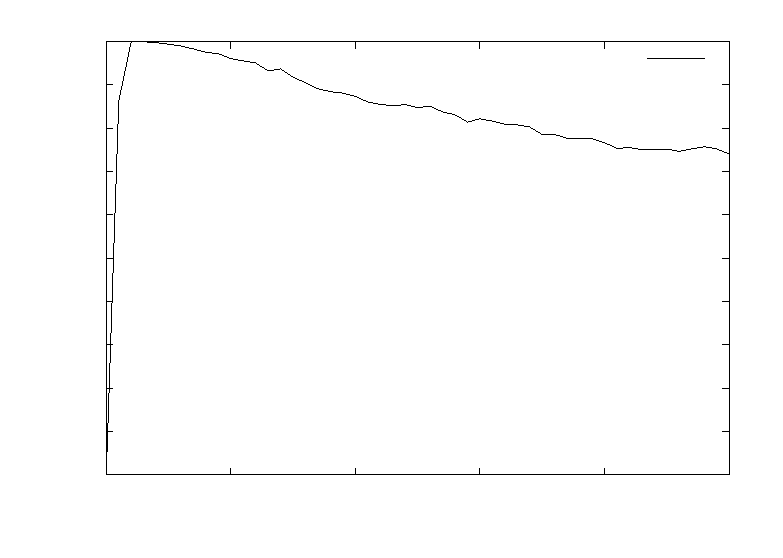
\includegraphics{chapters/chapter6/graphs/robustness/specializationratioovertime}}%
    \gplfronttext
  \end{picture}%
\endgroup
}
\caption{Specialization Ratio, $\tau$, of the honey bee algorithm, over time, when $\tau=0$ and $r=0.75$}
\label{fig:specializationratioovertime}
\end{figure}


\subsection{Flexibility in terms of Environment Distributions}
\label{results:flexibility:environmentdistribution}


An algorithm whose efficiency is the least affected by changes in environment distribution is considered to be the most flexible. The performance measure, $F_{ED}$ captures how efficiency is affected by changes in environment distributions. The lower the value of $F_{ED}$ is, the more flexible an algorithm is. The results presented in Table~\ref{table:flexibility} indicate that the honey bee algorithm was the most flexible, followed by the desert ant algorithm, in terms of environment distributions. The na\"ive algorithm was the least flexible.

%TODO: Hypothesis

The above suggests the following hypothesis:

The honey bees ability to adapt $\tau$ (described in Section~\ref{honeybeeforaging}) enables the honey bee algorithm to adapt the swarm specialization ratio, $\tau$, to more efficiently forage the differing environment ratios of the accessible environment (refer to Section~\ref{accessibleenvironment}) as the accessible environment changes throughout foraging.

To provide evidence for this hypothesis, an in-depth examination of each algorithm is performed, on a Gaussian environment, of high density or items, which has a low ratio of prioritized items and a swarm which has a high initial swarm specialization ratio (i.e. most robots are initially set to forage prioritized items). Since the non-prioritized items surround the prioritized items, the swarm should first forage the non-prioritized items in order to get access to the prioritized items. Once the swarm can reach the prioritized items, the swarm should switch to foraging the prioritized items. The example Gaussian environment is illustrated in Figure~\ref{fig:gaussianhighdensityenv}. The white cells represent an empty cell, the dark cells represent the cells containing a non-prioritized item and the shaded cells represent the cells containing a prioritized item. The environment in Figure~\ref{fig:gaussianhighdensityenv} has the following properties:

\begin{itemize}
\item A Gaussian environment item distribution,
\item a low environmental item ratio of $r=0.2$.
\item a high density of items $p=90$, and
\item an environment size $S=100$.
\end{itemize}

\begin{figure}[!htb]
\centering
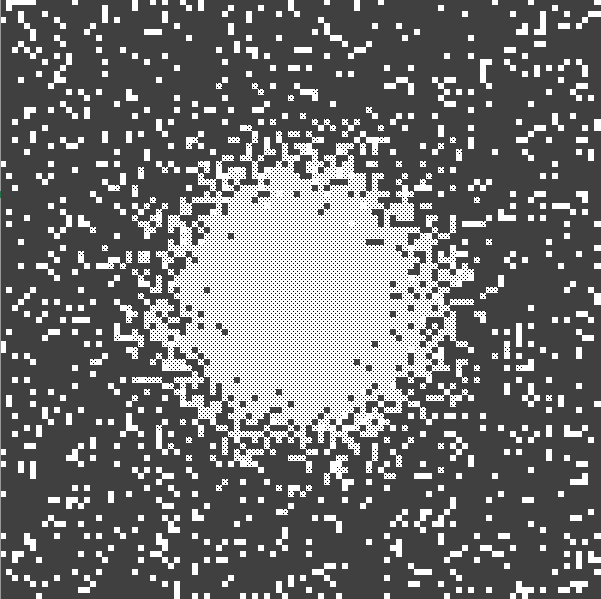
\includegraphics[width=0.75\textwidth]{chapters/chapter6/figures/flexibility-gaussian-obj90-ratio.PNG}
\caption{Gaussian environment with environment item type ratio, $r=0.2$, environment item density of $p=0.9$, and environment size $S=100$}
\label{fig:gaussianhighdensityenv}
\end{figure}

Also, consider a swarm with the initial specialization ratio set to mostly forage prioritized items (i.e. $\tau=0.8$) and with swarm density set to 0.5. The items nearest to the sink are all non-prioritized items. Robots will have to forage a large portion the non-prioritized items between the sink and the centre of the environment in order to reach the high density of prioritized items at the centre of the environment. 


So, figure~\ref{fig:gaussianhighdensityperformancehoneybee} shows the efficiency of foraging prioritized items $E_P$, the efficiency of foraging non-prioritized items $E_{NP}$, as well as the specialization ratio, $\tau$, for the honey bee algorithm, in 200 timestep intervals, on the Gaussian environment and swarm parameters described above, averaged over 30 independant runs.


\begin{figure}[!htb]
\centering
\small
\resizebox{\textwidth}{!}{% GNUPLOT: LaTeX picture with Postscript
\begingroup
  \makeatletter
  \providecommand\color[2][]{%
    \GenericError{(gnuplot) \space\space\space\@spaces}{%
      Package color not loaded in conjunction with
      terminal option `colourtext'%
    }{See the gnuplot documentation for explanation.%
    }{Either use 'blacktext' in gnuplot or load the package
      color.sty in LaTeX.}%
    \renewcommand\color[2][]{}%
  }%
  \providecommand\includegraphics[2][]{%
    \GenericError{(gnuplot) \space\space\space\@spaces}{%
      Package graphicx or graphics not loaded%
    }{See the gnuplot documentation for explanation.%
    }{The gnuplot epslatex terminal needs graphicx.sty or graphics.sty.}%
    \renewcommand\includegraphics[2][]{}%
  }%
  \providecommand\rotatebox[2]{#2}%
  \@ifundefined{ifGPcolor}{%
    \newif\ifGPcolor
    \GPcolorfalse
  }{}%
  \@ifundefined{ifGPblacktext}{%
    \newif\ifGPblacktext
    \GPblacktexttrue
  }{}%
  % define a \g@addto@macro without @ in the name:
  \let\gplgaddtomacro\g@addto@macro
  % define empty templates for all commands taking text:
  \gdef\gplbacktext{}%
  \gdef\gplfronttext{}%
  \makeatother
  \ifGPblacktext
    % no textcolor at all
    \def\colorrgb#1{}%
    \def\colorgray#1{}%
  \else
    % gray or color?
    \ifGPcolor
      \def\colorrgb#1{\color[rgb]{#1}}%
      \def\colorgray#1{\color[gray]{#1}}%
      \expandafter\def\csname LTw\endcsname{\color{white}}%
      \expandafter\def\csname LTb\endcsname{\color{black}}%
      \expandafter\def\csname LTa\endcsname{\color{black}}%
      \expandafter\def\csname LT0\endcsname{\color[rgb]{1,0,0}}%
      \expandafter\def\csname LT1\endcsname{\color[rgb]{0,1,0}}%
      \expandafter\def\csname LT2\endcsname{\color[rgb]{0,0,1}}%
      \expandafter\def\csname LT3\endcsname{\color[rgb]{1,0,1}}%
      \expandafter\def\csname LT4\endcsname{\color[rgb]{0,1,1}}%
      \expandafter\def\csname LT5\endcsname{\color[rgb]{1,1,0}}%
      \expandafter\def\csname LT6\endcsname{\color[rgb]{0,0,0}}%
      \expandafter\def\csname LT7\endcsname{\color[rgb]{1,0.3,0}}%
      \expandafter\def\csname LT8\endcsname{\color[rgb]{0.5,0.5,0.5}}%
    \else
      % gray
      \def\colorrgb#1{\color{black}}%
      \def\colorgray#1{\color[gray]{#1}}%
      \expandafter\def\csname LTw\endcsname{\color{white}}%
      \expandafter\def\csname LTb\endcsname{\color{black}}%
      \expandafter\def\csname LTa\endcsname{\color{black}}%
      \expandafter\def\csname LT0\endcsname{\color{black}}%
      \expandafter\def\csname LT1\endcsname{\color{black}}%
      \expandafter\def\csname LT2\endcsname{\color{black}}%
      \expandafter\def\csname LT3\endcsname{\color{black}}%
      \expandafter\def\csname LT4\endcsname{\color{black}}%
      \expandafter\def\csname LT5\endcsname{\color{black}}%
      \expandafter\def\csname LT6\endcsname{\color{black}}%
      \expandafter\def\csname LT7\endcsname{\color{black}}%
      \expandafter\def\csname LT8\endcsname{\color{black}}%
    \fi
  \fi
    \setlength{\unitlength}{0.0500bp}%
    \ifx\gptboxheight\undefined%
      \newlength{\gptboxheight}%
      \newlength{\gptboxwidth}%
      \newsavebox{\gptboxtext}%
    \fi%
    \setlength{\fboxrule}{0.5pt}%
    \setlength{\fboxsep}{1pt}%
\begin{picture}(7200.00,5040.00)%
    \gplgaddtomacro\gplbacktext{%
      \csname LTb\endcsname%
      \put(740,640){\makebox(0,0)[r]{\strut{}$0$}}%
      \put(740,1020){\makebox(0,0)[r]{\strut{}$10$}}%
      \put(740,1400){\makebox(0,0)[r]{\strut{}$20$}}%
      \put(740,1780){\makebox(0,0)[r]{\strut{}$30$}}%
      \put(740,2160){\makebox(0,0)[r]{\strut{}$40$}}%
      \put(740,2540){\makebox(0,0)[r]{\strut{}$50$}}%
      \put(740,2919){\makebox(0,0)[r]{\strut{}$60$}}%
      \put(740,3299){\makebox(0,0)[r]{\strut{}$70$}}%
      \put(740,3679){\makebox(0,0)[r]{\strut{}$80$}}%
      \put(740,4059){\makebox(0,0)[r]{\strut{}$90$}}%
      \put(740,4439){\makebox(0,0)[r]{\strut{}$100$}}%
      \put(860,440){\makebox(0,0){\strut{}$0$}}%
      \put(1896,440){\makebox(0,0){\strut{}$2000$}}%
      \put(2932,440){\makebox(0,0){\strut{}$4000$}}%
      \put(3967,440){\makebox(0,0){\strut{}$6000$}}%
      \put(5003,440){\makebox(0,0){\strut{}$8000$}}%
      \put(6039,440){\makebox(0,0){\strut{}$10000$}}%
      \put(6159,640){\makebox(0,0)[l]{\strut{}$0$}}%
      \put(6159,1020){\makebox(0,0)[l]{\strut{}$0.1$}}%
      \put(6159,1400){\makebox(0,0)[l]{\strut{}$0.2$}}%
      \put(6159,1780){\makebox(0,0)[l]{\strut{}$0.3$}}%
      \put(6159,2160){\makebox(0,0)[l]{\strut{}$0.4$}}%
      \put(6159,2540){\makebox(0,0)[l]{\strut{}$0.5$}}%
      \put(6159,2919){\makebox(0,0)[l]{\strut{}$0.6$}}%
      \put(6159,3299){\makebox(0,0)[l]{\strut{}$0.7$}}%
      \put(6159,3679){\makebox(0,0)[l]{\strut{}$0.8$}}%
      \put(6159,4059){\makebox(0,0)[l]{\strut{}$0.9$}}%
      \put(6159,4439){\makebox(0,0)[l]{\strut{}$1$}}%
    }%
    \gplgaddtomacro\gplfronttext{%
      \csname LTb\endcsname%
      \put(160,2539){\rotatebox{-270}{\makebox(0,0){\strut{}Efficiency ($E_P$ and $E_{NP}$)}}}%
      \put(6738,2539){\rotatebox{-270}{\makebox(0,0){\strut{}Specialiation ratio, $\tau$}}}%
      \put(3449,140){\makebox(0,0){\strut{}time steps}}%
      \put(5136,4276){\makebox(0,0)[r]{\strut{}$E_P$}}%
      \put(5136,4076){\makebox(0,0)[r]{\strut{}$E_{NP}$}}%
      \put(5136,3876){\makebox(0,0)[r]{\strut{}$\tau$}}%
    }%
    \gplbacktext
    \put(0,0){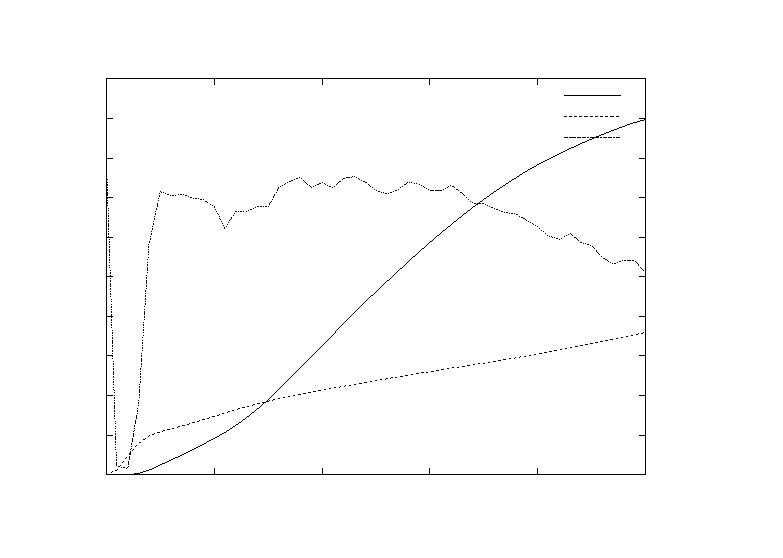
\includegraphics{chapters/chapter6/graphs/flexibility/flexibility-ED-gaussian-honeybee}}%
    \gplfronttext
  \end{picture}%
\endgroup
}
\caption{Efficiency of prioritized item foraging, $E_P$, efficiency of non-prioritized item foraging, $E_{NP}$, and specialization ratio over time, $\tau(t)$, for the honey bee algorithm on an example Gaussian environment, averaged over 30 independant runs}
\label{fig:gaussianhighdensityperformancehoneybee}
\end{figure}

In the first 200 timesteps, the efficiency of foraging nonprioritized items, $E_{NP}$, increased very slowly since there were very few robots that could forage non-prioritized items, because most of them were initialized to forage prioritized items. The efficiency of foraging prioritized items, E_{P}, did not increase in the first 200 timesteps, because the robots had no access to the prioritized items as they were blocked by the non-prioritized items. The specialization ratio $\tau$ that was initialized at 0.8, decreased very quickly to close to 0 in the first 200 time steps. The decrease in specialization ratio is good, because then most robots switched to forage non-prioritized items in the accessible environment which consisted entirely of non-prioritized items. Between 200 and 800 timesteps, due to the change in the swarm specialization ratio, the $E_{NP}$ increased very quickly, because most of the robots switched to foraging non-prioritized items. The E_{P} remained low between 200 and 800 timesteps, because the prioritized items were not yet accessible to the swarm. After 800 timesteps, $\tau$ increased from near 0 to just above 0.7, suggesting that the non-prioritized items have been cleared and the concentration of prioritized items in the centre have been reached. Thus most of robots in the swarm switched from foraging non-prioritized items to foraging prioritized items. The increase in swarm specialization ratio after 800 timesteps was followed by a sharp increase in $E_P$. This demonstrated that the honey bee algorithm could adapt $\tau$ in order to initially forage the large amount of non-prioritized items, and then switched to foraging mostly prioritized items when the prioritized items became accessible.

In constrast, the na\"ive algorithm's performance suffered because it lacks the ability to adapt swarm specialization. Figure~\ref{fig:gaussianhighdensityperformancenaive} illustrates the same performance measures, on the same Gaussian environment and swarm parameters. 

Because the na\"ive algorithm does not enable robots to switch their item specialization, the swarm specialization ratio, $\tau$ remains constant. Because so few robots could clear non-prioritized items, due to the large initial swarm specialization ratio, $E_{NP}$ increased slowly throughout the experiment. Because the swarm was slow to clear the non-prioritized items, the $E_P$ also remained small throughout the experiment, since the swarm struggled to make the prioritized items easily accessible. This suggests that prioritized foraging robots experienced environmental interference while attempting to navigate around the unforaged non-prioritized items. The rate of increase of $E_P$ increased over the duration of the experiment, as the swarm cleared more of the non-prioritized items. The behaviour for the desert ant algorithm was similar to that of the na\"ive algorithm, except that the final efficiency was greater for the desert ant algorithm.


Figure~\ref{fig:gaussianhighdensityperformancehoneybee} shows that final $E_P$ for the honey bee algorithm, averaged over 30 independant runs, was 0.9, while Figure~\ref{fig:gaussianhighdensityperformancenaive} shows that the final $E_P$ for the na\"ive algorithm was only 0.3. Since the honey bee algorithm adapts $\tau$, the honey bee algorithm shows an increased ability to forage obstacles (the non-prioritized items), in order to more easily access hard to reach prioritized items. As a result, the honey bee algorithm is more flexible too different environment distributions, than the na\"ive or desert ant algorithms.

\begin{figure}[!htb]
\centering
\small
\resizebox{\textwidth}{!}{% GNUPLOT: LaTeX picture with Postscript
\begingroup
  \makeatletter
  \providecommand\color[2][]{%
    \GenericError{(gnuplot) \space\space\space\@spaces}{%
      Package color not loaded in conjunction with
      terminal option `colourtext'%
    }{See the gnuplot documentation for explanation.%
    }{Either use 'blacktext' in gnuplot or load the package
      color.sty in LaTeX.}%
    \renewcommand\color[2][]{}%
  }%
  \providecommand\includegraphics[2][]{%
    \GenericError{(gnuplot) \space\space\space\@spaces}{%
      Package graphicx or graphics not loaded%
    }{See the gnuplot documentation for explanation.%
    }{The gnuplot epslatex terminal needs graphicx.sty or graphics.sty.}%
    \renewcommand\includegraphics[2][]{}%
  }%
  \providecommand\rotatebox[2]{#2}%
  \@ifundefined{ifGPcolor}{%
    \newif\ifGPcolor
    \GPcolorfalse
  }{}%
  \@ifundefined{ifGPblacktext}{%
    \newif\ifGPblacktext
    \GPblacktexttrue
  }{}%
  % define a \g@addto@macro without @ in the name:
  \let\gplgaddtomacro\g@addto@macro
  % define empty templates for all commands taking text:
  \gdef\gplbacktext{}%
  \gdef\gplfronttext{}%
  \makeatother
  \ifGPblacktext
    % no textcolor at all
    \def\colorrgb#1{}%
    \def\colorgray#1{}%
  \else
    % gray or color?
    \ifGPcolor
      \def\colorrgb#1{\color[rgb]{#1}}%
      \def\colorgray#1{\color[gray]{#1}}%
      \expandafter\def\csname LTw\endcsname{\color{white}}%
      \expandafter\def\csname LTb\endcsname{\color{black}}%
      \expandafter\def\csname LTa\endcsname{\color{black}}%
      \expandafter\def\csname LT0\endcsname{\color[rgb]{1,0,0}}%
      \expandafter\def\csname LT1\endcsname{\color[rgb]{0,1,0}}%
      \expandafter\def\csname LT2\endcsname{\color[rgb]{0,0,1}}%
      \expandafter\def\csname LT3\endcsname{\color[rgb]{1,0,1}}%
      \expandafter\def\csname LT4\endcsname{\color[rgb]{0,1,1}}%
      \expandafter\def\csname LT5\endcsname{\color[rgb]{1,1,0}}%
      \expandafter\def\csname LT6\endcsname{\color[rgb]{0,0,0}}%
      \expandafter\def\csname LT7\endcsname{\color[rgb]{1,0.3,0}}%
      \expandafter\def\csname LT8\endcsname{\color[rgb]{0.5,0.5,0.5}}%
    \else
      % gray
      \def\colorrgb#1{\color{black}}%
      \def\colorgray#1{\color[gray]{#1}}%
      \expandafter\def\csname LTw\endcsname{\color{white}}%
      \expandafter\def\csname LTb\endcsname{\color{black}}%
      \expandafter\def\csname LTa\endcsname{\color{black}}%
      \expandafter\def\csname LT0\endcsname{\color{black}}%
      \expandafter\def\csname LT1\endcsname{\color{black}}%
      \expandafter\def\csname LT2\endcsname{\color{black}}%
      \expandafter\def\csname LT3\endcsname{\color{black}}%
      \expandafter\def\csname LT4\endcsname{\color{black}}%
      \expandafter\def\csname LT5\endcsname{\color{black}}%
      \expandafter\def\csname LT6\endcsname{\color{black}}%
      \expandafter\def\csname LT7\endcsname{\color{black}}%
      \expandafter\def\csname LT8\endcsname{\color{black}}%
    \fi
  \fi
    \setlength{\unitlength}{0.0500bp}%
    \ifx\gptboxheight\undefined%
      \newlength{\gptboxheight}%
      \newlength{\gptboxwidth}%
      \newsavebox{\gptboxtext}%
    \fi%
    \setlength{\fboxrule}{0.5pt}%
    \setlength{\fboxsep}{1pt}%
\begin{picture}(7200.00,5040.00)%
    \gplgaddtomacro\gplbacktext{%
      \csname LTb\endcsname%
      \put(740,640){\makebox(0,0)[r]{\strut{}$0$}}%
      \put(740,1056){\makebox(0,0)[r]{\strut{}$10$}}%
      \put(740,1472){\makebox(0,0)[r]{\strut{}$20$}}%
      \put(740,1888){\makebox(0,0)[r]{\strut{}$30$}}%
      \put(740,2304){\makebox(0,0)[r]{\strut{}$40$}}%
      \put(740,2720){\makebox(0,0)[r]{\strut{}$50$}}%
      \put(740,3135){\makebox(0,0)[r]{\strut{}$60$}}%
      \put(740,3551){\makebox(0,0)[r]{\strut{}$70$}}%
      \put(740,3967){\makebox(0,0)[r]{\strut{}$80$}}%
      \put(740,4383){\makebox(0,0)[r]{\strut{}$90$}}%
      \put(740,4799){\makebox(0,0)[r]{\strut{}$100$}}%
      \put(860,440){\makebox(0,0){\strut{}$0$}}%
      \put(1896,440){\makebox(0,0){\strut{}$2000$}}%
      \put(2932,440){\makebox(0,0){\strut{}$4000$}}%
      \put(3967,440){\makebox(0,0){\strut{}$6000$}}%
      \put(5003,440){\makebox(0,0){\strut{}$8000$}}%
      \put(6039,440){\makebox(0,0){\strut{}$10000$}}%
      \put(6159,640){\makebox(0,0)[l]{\strut{}$0$}}%
      \put(6159,1056){\makebox(0,0)[l]{\strut{}$0.1$}}%
      \put(6159,1472){\makebox(0,0)[l]{\strut{}$0.2$}}%
      \put(6159,1888){\makebox(0,0)[l]{\strut{}$0.3$}}%
      \put(6159,2304){\makebox(0,0)[l]{\strut{}$0.4$}}%
      \put(6159,2720){\makebox(0,0)[l]{\strut{}$0.5$}}%
      \put(6159,3135){\makebox(0,0)[l]{\strut{}$0.6$}}%
      \put(6159,3551){\makebox(0,0)[l]{\strut{}$0.7$}}%
      \put(6159,3967){\makebox(0,0)[l]{\strut{}$0.8$}}%
      \put(6159,4383){\makebox(0,0)[l]{\strut{}$0.9$}}%
      \put(6159,4799){\makebox(0,0)[l]{\strut{}$1$}}%
    }%
    \gplgaddtomacro\gplfronttext{%
      \csname LTb\endcsname%
      \put(160,2719){\rotatebox{-270}{\makebox(0,0){\strut{}Efficiency}}}%
      \put(6738,2719){\rotatebox{-270}{\makebox(0,0){\strut{}Specialiation ratio, $\tau$}}}%
      \put(3449,140){\makebox(0,0){\strut{}time steps}}%
      \put(5136,4636){\makebox(0,0)[r]{\strut{}$E_P$}}%
      \put(5136,4436){\makebox(0,0)[r]{\strut{}$E_{NP}$}}%
      \put(5136,4236){\makebox(0,0)[r]{\strut{}$\tau$}}%
    }%
    \gplbacktext
    \put(0,0){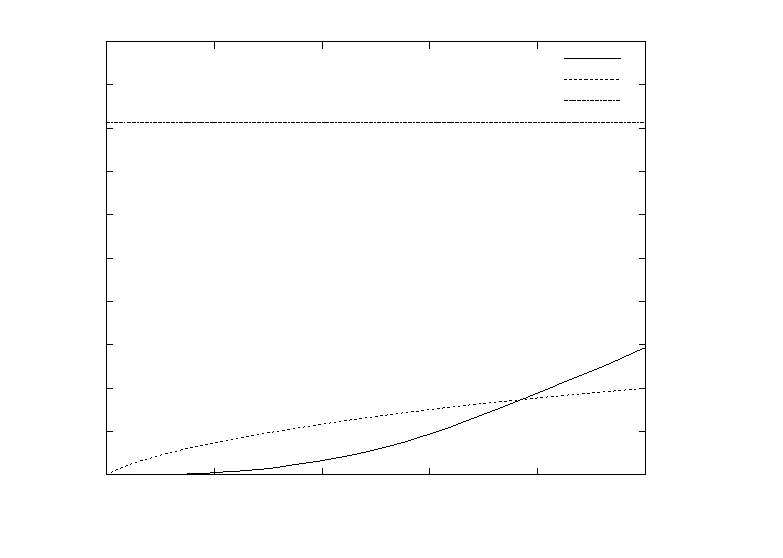
\includegraphics{chapters/chapter6/graphs/flexibility/flexibility-ED-gaussian-naive}}%
    \gplfronttext
  \end{picture}%
\endgroup
}
\caption{Efficiency of prioritized item foraging $E_P$, efficiency of non-prioritized item foraging $E_{NP}$, and the specialization ratio over time $\tau$, for the na\"ive algorithm on a Gaussian evironment, averaged over 30 independant runs}
\label{fig:gaussianhighdensityperformancenaive}
\end{figure}

\begin{figure}[!htb]
\centering
\small
\resizebox{\textwidth}{!}{% GNUPLOT: LaTeX picture with Postscript
\begingroup
  \makeatletter
  \providecommand\color[2][]{%
    \GenericError{(gnuplot) \space\space\space\@spaces}{%
      Package color not loaded in conjunction with
      terminal option `colourtext'%
    }{See the gnuplot documentation for explanation.%
    }{Either use 'blacktext' in gnuplot or load the package
      color.sty in LaTeX.}%
    \renewcommand\color[2][]{}%
  }%
  \providecommand\includegraphics[2][]{%
    \GenericError{(gnuplot) \space\space\space\@spaces}{%
      Package graphicx or graphics not loaded%
    }{See the gnuplot documentation for explanation.%
    }{The gnuplot epslatex terminal needs graphicx.sty or graphics.sty.}%
    \renewcommand\includegraphics[2][]{}%
  }%
  \providecommand\rotatebox[2]{#2}%
  \@ifundefined{ifGPcolor}{%
    \newif\ifGPcolor
    \GPcolorfalse
  }{}%
  \@ifundefined{ifGPblacktext}{%
    \newif\ifGPblacktext
    \GPblacktexttrue
  }{}%
  % define a \g@addto@macro without @ in the name:
  \let\gplgaddtomacro\g@addto@macro
  % define empty templates for all commands taking text:
  \gdef\gplbacktext{}%
  \gdef\gplfronttext{}%
  \makeatother
  \ifGPblacktext
    % no textcolor at all
    \def\colorrgb#1{}%
    \def\colorgray#1{}%
  \else
    % gray or color?
    \ifGPcolor
      \def\colorrgb#1{\color[rgb]{#1}}%
      \def\colorgray#1{\color[gray]{#1}}%
      \expandafter\def\csname LTw\endcsname{\color{white}}%
      \expandafter\def\csname LTb\endcsname{\color{black}}%
      \expandafter\def\csname LTa\endcsname{\color{black}}%
      \expandafter\def\csname LT0\endcsname{\color[rgb]{1,0,0}}%
      \expandafter\def\csname LT1\endcsname{\color[rgb]{0,1,0}}%
      \expandafter\def\csname LT2\endcsname{\color[rgb]{0,0,1}}%
      \expandafter\def\csname LT3\endcsname{\color[rgb]{1,0,1}}%
      \expandafter\def\csname LT4\endcsname{\color[rgb]{0,1,1}}%
      \expandafter\def\csname LT5\endcsname{\color[rgb]{1,1,0}}%
      \expandafter\def\csname LT6\endcsname{\color[rgb]{0,0,0}}%
      \expandafter\def\csname LT7\endcsname{\color[rgb]{1,0.3,0}}%
      \expandafter\def\csname LT8\endcsname{\color[rgb]{0.5,0.5,0.5}}%
    \else
      % gray
      \def\colorrgb#1{\color{black}}%
      \def\colorgray#1{\color[gray]{#1}}%
      \expandafter\def\csname LTw\endcsname{\color{white}}%
      \expandafter\def\csname LTb\endcsname{\color{black}}%
      \expandafter\def\csname LTa\endcsname{\color{black}}%
      \expandafter\def\csname LT0\endcsname{\color{black}}%
      \expandafter\def\csname LT1\endcsname{\color{black}}%
      \expandafter\def\csname LT2\endcsname{\color{black}}%
      \expandafter\def\csname LT3\endcsname{\color{black}}%
      \expandafter\def\csname LT4\endcsname{\color{black}}%
      \expandafter\def\csname LT5\endcsname{\color{black}}%
      \expandafter\def\csname LT6\endcsname{\color{black}}%
      \expandafter\def\csname LT7\endcsname{\color{black}}%
      \expandafter\def\csname LT8\endcsname{\color{black}}%
    \fi
  \fi
    \setlength{\unitlength}{0.0500bp}%
    \ifx\gptboxheight\undefined%
      \newlength{\gptboxheight}%
      \newlength{\gptboxwidth}%
      \newsavebox{\gptboxtext}%
    \fi%
    \setlength{\fboxrule}{0.5pt}%
    \setlength{\fboxsep}{1pt}%
\begin{picture}(7200.00,5040.00)%
    \gplgaddtomacro\gplbacktext{%
      \csname LTb\endcsname%
      \put(740,640){\makebox(0,0)[r]{\strut{}$0$}}%
      \put(740,1020){\makebox(0,0)[r]{\strut{}$10$}}%
      \put(740,1400){\makebox(0,0)[r]{\strut{}$20$}}%
      \put(740,1780){\makebox(0,0)[r]{\strut{}$30$}}%
      \put(740,2160){\makebox(0,0)[r]{\strut{}$40$}}%
      \put(740,2540){\makebox(0,0)[r]{\strut{}$50$}}%
      \put(740,2919){\makebox(0,0)[r]{\strut{}$60$}}%
      \put(740,3299){\makebox(0,0)[r]{\strut{}$70$}}%
      \put(740,3679){\makebox(0,0)[r]{\strut{}$80$}}%
      \put(740,4059){\makebox(0,0)[r]{\strut{}$90$}}%
      \put(740,4439){\makebox(0,0)[r]{\strut{}$100$}}%
      \put(860,440){\makebox(0,0){\strut{}$0$}}%
      \put(1896,440){\makebox(0,0){\strut{}$2000$}}%
      \put(2932,440){\makebox(0,0){\strut{}$4000$}}%
      \put(3967,440){\makebox(0,0){\strut{}$6000$}}%
      \put(5003,440){\makebox(0,0){\strut{}$8000$}}%
      \put(6039,440){\makebox(0,0){\strut{}$10000$}}%
      \put(6159,640){\makebox(0,0)[l]{\strut{}$0$}}%
      \put(6159,1020){\makebox(0,0)[l]{\strut{}$0.1$}}%
      \put(6159,1400){\makebox(0,0)[l]{\strut{}$0.2$}}%
      \put(6159,1780){\makebox(0,0)[l]{\strut{}$0.3$}}%
      \put(6159,2160){\makebox(0,0)[l]{\strut{}$0.4$}}%
      \put(6159,2540){\makebox(0,0)[l]{\strut{}$0.5$}}%
      \put(6159,2919){\makebox(0,0)[l]{\strut{}$0.6$}}%
      \put(6159,3299){\makebox(0,0)[l]{\strut{}$0.7$}}%
      \put(6159,3679){\makebox(0,0)[l]{\strut{}$0.8$}}%
      \put(6159,4059){\makebox(0,0)[l]{\strut{}$0.9$}}%
      \put(6159,4439){\makebox(0,0)[l]{\strut{}$1$}}%
    }%
    \gplgaddtomacro\gplfronttext{%
      \csname LTb\endcsname%
      \put(160,2539){\rotatebox{-270}{\makebox(0,0){\strut{}Efficiency}}}%
      \put(6738,2539){\rotatebox{-270}{\makebox(0,0){\strut{}Specialiation ratio, $\tau$}}}%
      \put(3449,140){\makebox(0,0){\strut{}iteration}}%
      \put(3449,4739){\makebox(0,0){\strut{}Efficiency of prioritized item foraging $E_P$, Efficiency of non-prioritized item foraging $E_{NP}$, Specialization ratio $\tau$ over time, for Honey Bee in Uniform Environment}}%
      \put(5136,4276){\makebox(0,0)[r]{\strut{}$E_P$}}%
      \put(5136,4076){\makebox(0,0)[r]{\strut{}$E_{NP}$}}%
      \put(5136,3876){\makebox(0,0)[r]{\strut{}$\tau$}}%
    }%
    \gplbacktext
    \put(0,0){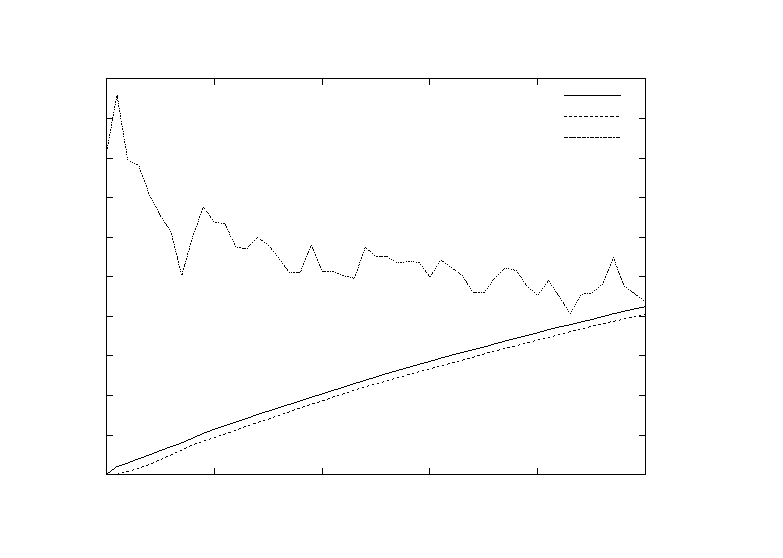
\includegraphics{chapters/chapter6/graphs/flexibility/flexibility-ED-uniform-honeybee}}%
    \gplfronttext
  \end{picture}%
\endgroup
}
\caption{Efficiency of prioritized item foraging $E_P$ over time $t$, efficiency of non-prioritized item foraging $E_{NP}$ over time $t$, and specialization ratio $\tau(t)$, for the honey bee algorithm on a uniform environment, averaged over 30 independant runs}
\label{fig:uniformhighdensityperformancehoneybee}
\end{figure}


To provide further evidence for the above hypothesis, one must consider other environment distributions, to show that honey bee algorithm can adapt the swarm's $\tau$ appropriately, for different distributions. Thus, consider a uniform environment with the same environment parameters as above. Because the environment distribution is uniform, environment ratio of the accessible environment will fluctuate erratically as the swarm forages the environment.  

Figure~\ref{fig:uniformhighdensityperformancehoneybee} shows the same performance measures, for an experiment with the same swarm parameters as above on the uniform environment, for the honey bee algorithm. The specialization ratio has a downward erratic trend, from over 0.9 to approximately 0.4. The erratic fluctuation of $\tau$ is due to minor and short-lived erratic differences in the environment ratio of the accessible environment which would feature in uniform environments. The rate of foraging efficiency $E_P$ and $E_{NP}$  increase constantly throughout the experiment. 

The above analysis provides evidence for the hypothesis that suggests that the honey bee algorithm is capable of adapting the swarm to forage the accessible environment which results in improved flexibility on different environment distributions, where as the desert ant and na\"ive algorithms have more difficulty foraging certain distributions as they cannot adapt $
tau$ to more effectively forage the accessible environment.

Table~\ref{table:flexibility} indicates that desert ant algorithm is more flexible over environment distributions than the the na\"ive algorithm. Considering the fact that the only difference between the na\"ive algorithm and the desert ant algorithm, is the fact that the desert ant algorithm uses site fidelity while the na\"ive algorithm does not, the difference must be attributed to the desert ant's use of site fidelity. %TODO: How about we examine the vein environment? Dessert ant could use site fidelity. 

\section{Scalability}
\label{results:scalability}

This section discusses the scalability of each algorithm in terms of the macro performance measures in terms of swarm density and problem complexity. Section~\ref{results:swarmscalability} discusses scalability of each algorithm, in terms of swarm density while Section~\ref{results:problemscalability} discusses the scalability of each algorithm, in terms of the complexity of the problem.

\subsection{Swarm scalability}
\label{results:swarmscalability}
Table~\ref{table:swarmscalability} present the swarm density scalability results, $SS$. Figure~\ref{fig:swarmscalability}, show the swarm density scalability for each density, $SS_c$, for each algorithm (as defined Section~\ref{swarmsizescalability}). The na\"ive algorithm was the most scalable while the desert ant and the honey bee algorithms show similar scalability. The honey bee algorithm is scalable than the desert ant algorithm for $c < 0.9$, but at $c \geq 0.9$, the swarm scalability, $SS_c$, of the desert ant algorithm was greater than the honey bee algorithm.

\begin{table}[]
\centering
\caption{Swarm scalability, $SS$, for each swarm density, $c$, for each algorithm.}
\label{table:swarmscalability}
\begin{tabular}{@{}lllllll@{}}
\toprule
\textbf{$c$}            & \textbf{0.1} & \textbf{0.3}         & \textbf{0.5}         & \textbf{0.7}         & \textbf{1}           \\ \midrule
\textbf{na\"ive}    & 1   & 2.148309055 & 2.95067493  & 3.567754813 & 4.25529855  \\
\textbf{desert ant} & 1   & 1.972768821 & 2.604500744 & 3.05833543  & 3.555516648 \\
\textbf{honey bee}  & 1   & 2.067364168 & 2.706034502 & 3.119174449 & 3.532352867 \\ \bottomrule
\end{tabular}
\end{table}

\begin{figure}[!htb]
\centering
\small
\resizebox{\textwidth}{!}{% GNUPLOT: LaTeX picture with Postscript
\begingroup
  \makeatletter
  \providecommand\color[2][]{%
    \GenericError{(gnuplot) \space\space\space\@spaces}{%
      Package color not loaded in conjunction with
      terminal option `colourtext'%
    }{See the gnuplot documentation for explanation.%
    }{Either use 'blacktext' in gnuplot or load the package
      color.sty in LaTeX.}%
    \renewcommand\color[2][]{}%
  }%
  \providecommand\includegraphics[2][]{%
    \GenericError{(gnuplot) \space\space\space\@spaces}{%
      Package graphicx or graphics not loaded%
    }{See the gnuplot documentation for explanation.%
    }{The gnuplot epslatex terminal needs graphicx.sty or graphics.sty.}%
    \renewcommand\includegraphics[2][]{}%
  }%
  \providecommand\rotatebox[2]{#2}%
  \@ifundefined{ifGPcolor}{%
    \newif\ifGPcolor
    \GPcolorfalse
  }{}%
  \@ifundefined{ifGPblacktext}{%
    \newif\ifGPblacktext
    \GPblacktexttrue
  }{}%
  % define a \g@addto@macro without @ in the name:
  \let\gplgaddtomacro\g@addto@macro
  % define empty templates for all commands taking text:
  \gdef\gplbacktext{}%
  \gdef\gplfronttext{}%
  \makeatother
  \ifGPblacktext
    % no textcolor at all
    \def\colorrgb#1{}%
    \def\colorgray#1{}%
  \else
    % gray or color?
    \ifGPcolor
      \def\colorrgb#1{\color[rgb]{#1}}%
      \def\colorgray#1{\color[gray]{#1}}%
      \expandafter\def\csname LTw\endcsname{\color{white}}%
      \expandafter\def\csname LTb\endcsname{\color{black}}%
      \expandafter\def\csname LTa\endcsname{\color{black}}%
      \expandafter\def\csname LT0\endcsname{\color[rgb]{1,0,0}}%
      \expandafter\def\csname LT1\endcsname{\color[rgb]{0,1,0}}%
      \expandafter\def\csname LT2\endcsname{\color[rgb]{0,0,1}}%
      \expandafter\def\csname LT3\endcsname{\color[rgb]{1,0,1}}%
      \expandafter\def\csname LT4\endcsname{\color[rgb]{0,1,1}}%
      \expandafter\def\csname LT5\endcsname{\color[rgb]{1,1,0}}%
      \expandafter\def\csname LT6\endcsname{\color[rgb]{0,0,0}}%
      \expandafter\def\csname LT7\endcsname{\color[rgb]{1,0.3,0}}%
      \expandafter\def\csname LT8\endcsname{\color[rgb]{0.5,0.5,0.5}}%
    \else
      % gray
      \def\colorrgb#1{\color{black}}%
      \def\colorgray#1{\color[gray]{#1}}%
      \expandafter\def\csname LTw\endcsname{\color{white}}%
      \expandafter\def\csname LTb\endcsname{\color{black}}%
      \expandafter\def\csname LTa\endcsname{\color{black}}%
      \expandafter\def\csname LT0\endcsname{\color{black}}%
      \expandafter\def\csname LT1\endcsname{\color{black}}%
      \expandafter\def\csname LT2\endcsname{\color{black}}%
      \expandafter\def\csname LT3\endcsname{\color{black}}%
      \expandafter\def\csname LT4\endcsname{\color{black}}%
      \expandafter\def\csname LT5\endcsname{\color{black}}%
      \expandafter\def\csname LT6\endcsname{\color{black}}%
      \expandafter\def\csname LT7\endcsname{\color{black}}%
      \expandafter\def\csname LT8\endcsname{\color{black}}%
    \fi
  \fi
    \setlength{\unitlength}{0.0500bp}%
    \ifx\gptboxheight\undefined%
      \newlength{\gptboxheight}%
      \newlength{\gptboxwidth}%
      \newsavebox{\gptboxtext}%
    \fi%
    \setlength{\fboxrule}{0.5pt}%
    \setlength{\fboxsep}{1pt}%
\begin{picture}(7200.00,5040.00)%
    \gplgaddtomacro\gplbacktext{%
      \csname LTb\endcsname%
      \put(620,640){\makebox(0,0)[r]{\strut{}$1$}}%
      \put(620,1062){\makebox(0,0)[r]{\strut{}$2$}}%
      \put(620,1484){\makebox(0,0)[r]{\strut{}$3$}}%
      \put(620,1906){\makebox(0,0)[r]{\strut{}$4$}}%
      \put(620,2328){\makebox(0,0)[r]{\strut{}$5$}}%
      \put(620,2751){\makebox(0,0)[r]{\strut{}$6$}}%
      \put(620,3173){\makebox(0,0)[r]{\strut{}$7$}}%
      \put(620,3595){\makebox(0,0)[r]{\strut{}$8$}}%
      \put(620,4017){\makebox(0,0)[r]{\strut{}$9$}}%
      \put(620,4439){\makebox(0,0)[r]{\strut{}$10$}}%
      \put(740,440){\makebox(0,0){\strut{}$0.1$}}%
      \put(1418,440){\makebox(0,0){\strut{}$0.2$}}%
      \put(2095,440){\makebox(0,0){\strut{}$0.3$}}%
      \put(2773,440){\makebox(0,0){\strut{}$0.4$}}%
      \put(3451,440){\makebox(0,0){\strut{}$0.5$}}%
      \put(4128,440){\makebox(0,0){\strut{}$0.6$}}%
      \put(4806,440){\makebox(0,0){\strut{}$0.7$}}%
      \put(5484,440){\makebox(0,0){\strut{}$0.8$}}%
      \put(6161,440){\makebox(0,0){\strut{}$0.9$}}%
      \put(6839,440){\makebox(0,0){\strut{}$1$}}%
    }%
    \gplgaddtomacro\gplfronttext{%
      \csname LTb\endcsname%
      \put(160,2539){\rotatebox{-270}{\makebox(0,0){\strut{}Swarm Scalability ($SS$)}}}%
      \put(3789,140){\makebox(0,0){\strut{}swarm density ($c$)}}%
      \put(3789,4739){\makebox(0,0){\strut{}Swarm Scalability, $SS$, for each swarm density $c$, for each algorithm}}%
      \put(5936,4276){\makebox(0,0)[r]{\strut{}Na\"ive}}%
      \put(5936,4076){\makebox(0,0)[r]{\strut{}Desert Ant}}%
      \put(5936,3876){\makebox(0,0)[r]{\strut{}Honey Bee}}%
      \put(5936,3676){\makebox(0,0)[r]{\strut{}Linear Scalability}}%
    }%
    \gplbacktext
    \put(0,0){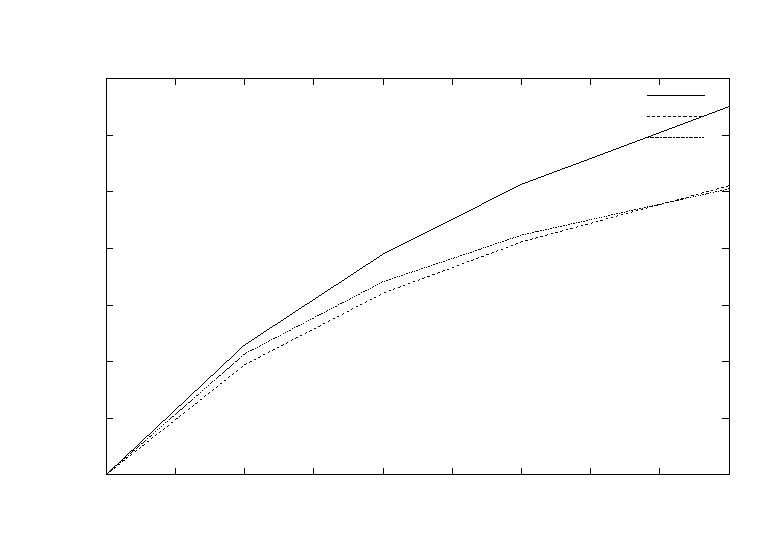
\includegraphics{chapters/chapter6/graphs/scalability/swarmscalability}}%
    \gplfronttext
  \end{picture}%
\endgroup
}
\caption{Swarm scalability, $SS$, for each swarm density $c$, for each algorithm.}
\label{fig:swarmscalability}
\end{figure}

Figure~\ref{fig:swarmscalability} also plots the ideal scalability. Ideal scalability is when the increase in swarm density is directly proportional to the increase in efficiency. Based on that, the ideal values for $SS_c$ were calculated and plotted. All algorithms fall below the ideal scalability line and thus have sublinear (logarithmic) scalability. Section~\ref{swarmsizescalability} highlighted that increased inter-robot interference is a major factor that impacts swarm scalability. It can be concluded that the reason for sub-linear performance in all algorithms was because all algorithms suffer from increased inter-robot interference as swarm size increases.

To understand why the desert ant and the honey bee algorithms were less scalable than the na\"ive algorithm, consider the following:

The na\"ive algorithm, being the most simple foraging algorithm, has no mechanism to enable the swarm to exploit high quality sites of prioritized items and can only locate items by randomly exploring the environment. Both the desert ant algorithm and the honey bee algorithm have mechanisms to exploit high quality areas: The desert ant algorithm uses site fidelity and the honey bee algorithm uses recruitment to exploit high quality sites. 

Suppose that there exists a single high quality site in an environment. Using site-fidelity and recruitment, the desert ant and the honey bee algorithms can exploit that high quality area. In exploiting that high quality site, the path between the sink and the high-quality site becomes more congested as more robots share the path between the sink and the high quality area. The increased congestion on that path will cause more inter-robot interference. However, due to the focused efforts of the swarm on a high quality area of the environment, the exploitation will still improve foraging efficiency overall, compared to the na\"ive algorithm at low swarm densities. However, as swarm density increases, the congestion on the route between the high quality site and the sink will increase, hindering the foraging efficiency due to increased greater inter-robot interference. It follows that the desert ant algorithm and the honey bee algorithm are less scalable in terms of swarm density than the na\"ive algorithm, due to the increased inter-robot interference as a result of exploitation of high quality sites.

The recruitment mechanism used by the honey bee algorithm is a more extreme form of exploitation than site fidelity used by the desert ant algorithm, because scouts recruit groups of robots to forage single areas. On the other hand, when using site fidelity, the high quality site is only foraged by the robot that found it. Considering that the recruitment mechanism is more exploitative than the site fidelity mechanism, one would expect the honey bee algorithm to be much less scalable than the desert ant algorithm, but that is not evidential in Table~\ref{table:swarmscalability}. Instead, the honey bee algorithm performed slightly better than the desert ant algorithm for all $c < 0.8$.

To explain the honey bee algorithm's ability to outperform the desert ant algorithm at most swarm densities, consider the honey bee algorithm's division of labour mechanism as described in Section~\ref{honeybeeforaging}. The division of labour mechanism will cause an active forager robot to return to the sink if that robot can not find an item for a maximum amount of time. The inactive forager robot waits at the sink, until the inactive forager robot is recruited by a scout robot. Section~\ref{background:divisionoflabour:robotswarm} discussed that a mechanism of division of labour, which could adjust the number of robots actively foraging to an appropriate number, would result in decreased levels of inter-robot interference and increased swarm scalability.

In order to determine whether the slight improvement in scalability of the honey bee algorithm over the desert ant algorithm can be attributed to the discussed division of labour mechanism, the average time spent by robots in the waiting state is plotted for different values of $c$ in Figure~\ref{fig:swarmscalabilitywaitingtime}. Figure~\ref{fig:swarmscalabilitywaitingtime} illustrates that the robots spend a significant portion of time in the waiting state for $c < 0.5$ which provides evidence that the honey bee algorithm's swarm scalability is greater than the desert ant algorithm's swarm scalability for low values of $c$.

\begin{figure}[!htb]
\centering
\small
\resizebox{\textwidth}{!}{% GNUPLOT: LaTeX picture with Postscript
\begingroup
  \makeatletter
  \providecommand\color[2][]{%
    \GenericError{(gnuplot) \space\space\space\@spaces}{%
      Package color not loaded in conjunction with
      terminal option `colourtext'%
    }{See the gnuplot documentation for explanation.%
    }{Either use 'blacktext' in gnuplot or load the package
      color.sty in LaTeX.}%
    \renewcommand\color[2][]{}%
  }%
  \providecommand\includegraphics[2][]{%
    \GenericError{(gnuplot) \space\space\space\@spaces}{%
      Package graphicx or graphics not loaded%
    }{See the gnuplot documentation for explanation.%
    }{The gnuplot epslatex terminal needs graphicx.sty or graphics.sty.}%
    \renewcommand\includegraphics[2][]{}%
  }%
  \providecommand\rotatebox[2]{#2}%
  \@ifundefined{ifGPcolor}{%
    \newif\ifGPcolor
    \GPcolorfalse
  }{}%
  \@ifundefined{ifGPblacktext}{%
    \newif\ifGPblacktext
    \GPblacktexttrue
  }{}%
  % define a \g@addto@macro without @ in the name:
  \let\gplgaddtomacro\g@addto@macro
  % define empty templates for all commands taking text:
  \gdef\gplbacktext{}%
  \gdef\gplfronttext{}%
  \makeatother
  \ifGPblacktext
    % no textcolor at all
    \def\colorrgb#1{}%
    \def\colorgray#1{}%
  \else
    % gray or color?
    \ifGPcolor
      \def\colorrgb#1{\color[rgb]{#1}}%
      \def\colorgray#1{\color[gray]{#1}}%
      \expandafter\def\csname LTw\endcsname{\color{white}}%
      \expandafter\def\csname LTb\endcsname{\color{black}}%
      \expandafter\def\csname LTa\endcsname{\color{black}}%
      \expandafter\def\csname LT0\endcsname{\color[rgb]{1,0,0}}%
      \expandafter\def\csname LT1\endcsname{\color[rgb]{0,1,0}}%
      \expandafter\def\csname LT2\endcsname{\color[rgb]{0,0,1}}%
      \expandafter\def\csname LT3\endcsname{\color[rgb]{1,0,1}}%
      \expandafter\def\csname LT4\endcsname{\color[rgb]{0,1,1}}%
      \expandafter\def\csname LT5\endcsname{\color[rgb]{1,1,0}}%
      \expandafter\def\csname LT6\endcsname{\color[rgb]{0,0,0}}%
      \expandafter\def\csname LT7\endcsname{\color[rgb]{1,0.3,0}}%
      \expandafter\def\csname LT8\endcsname{\color[rgb]{0.5,0.5,0.5}}%
    \else
      % gray
      \def\colorrgb#1{\color{black}}%
      \def\colorgray#1{\color[gray]{#1}}%
      \expandafter\def\csname LTw\endcsname{\color{white}}%
      \expandafter\def\csname LTb\endcsname{\color{black}}%
      \expandafter\def\csname LTa\endcsname{\color{black}}%
      \expandafter\def\csname LT0\endcsname{\color{black}}%
      \expandafter\def\csname LT1\endcsname{\color{black}}%
      \expandafter\def\csname LT2\endcsname{\color{black}}%
      \expandafter\def\csname LT3\endcsname{\color{black}}%
      \expandafter\def\csname LT4\endcsname{\color{black}}%
      \expandafter\def\csname LT5\endcsname{\color{black}}%
      \expandafter\def\csname LT6\endcsname{\color{black}}%
      \expandafter\def\csname LT7\endcsname{\color{black}}%
      \expandafter\def\csname LT8\endcsname{\color{black}}%
    \fi
  \fi
    \setlength{\unitlength}{0.0500bp}%
    \ifx\gptboxheight\undefined%
      \newlength{\gptboxheight}%
      \newlength{\gptboxwidth}%
      \newsavebox{\gptboxtext}%
    \fi%
    \setlength{\fboxrule}{0.5pt}%
    \setlength{\fboxsep}{1pt}%
\begin{picture}(7200.00,5040.00)%
    \gplgaddtomacro\gplbacktext{%
      \csname LTb\endcsname%
      \put(860,640){\makebox(0,0)[r]{\strut{}$0.05$}}%
      \put(860,1400){\makebox(0,0)[r]{\strut{}$0.1$}}%
      \put(860,2160){\makebox(0,0)[r]{\strut{}$0.15$}}%
      \put(860,2919){\makebox(0,0)[r]{\strut{}$0.2$}}%
      \put(860,3679){\makebox(0,0)[r]{\strut{}$0.25$}}%
      \put(860,4439){\makebox(0,0)[r]{\strut{}$0.3$}}%
      \put(980,440){\makebox(0,0){\strut{}$0.1$}}%
      \put(1631,440){\makebox(0,0){\strut{}$0.2$}}%
      \put(2282,440){\makebox(0,0){\strut{}$0.3$}}%
      \put(2933,440){\makebox(0,0){\strut{}$0.4$}}%
      \put(3584,440){\makebox(0,0){\strut{}$0.5$}}%
      \put(4235,440){\makebox(0,0){\strut{}$0.6$}}%
      \put(4886,440){\makebox(0,0){\strut{}$0.7$}}%
      \put(5537,440){\makebox(0,0){\strut{}$0.8$}}%
      \put(6188,440){\makebox(0,0){\strut{}$0.9$}}%
      \put(6839,440){\makebox(0,0){\strut{}$1$}}%
    }%
    \gplgaddtomacro\gplfronttext{%
      \csname LTb\endcsname%
      \put(160,2539){\rotatebox{-270}{\makebox(0,0){\strut{}Average Time in Waiting State ($t_{wait}$)}}}%
      \put(3909,140){\makebox(0,0){\strut{}swarm density ($c$)}}%
    }%
    \gplbacktext
    \put(0,0){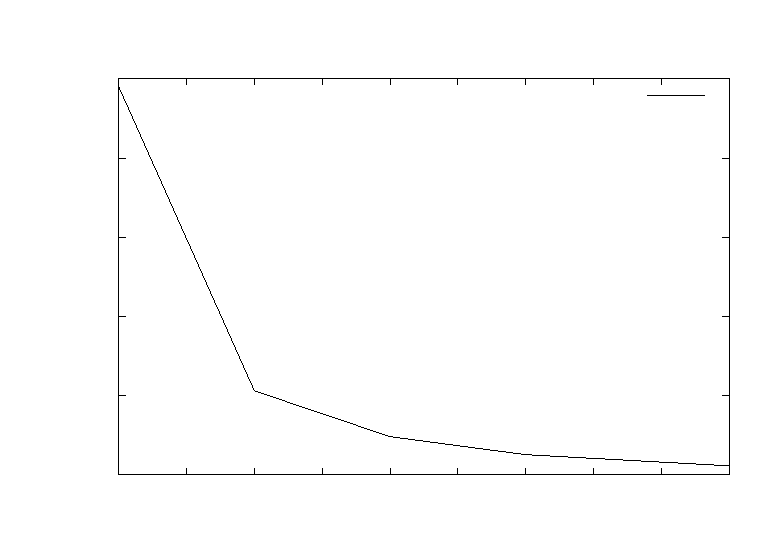
\includegraphics{chapters/chapter6/graphs/scalability/swarm-scalability-waitingtime}}%
    \gplfronttext
  \end{picture}%
\endgroup
}
\caption{Average time in waiting state, $t_{wait}$, for each swarm density $c$, for the honey bee algorithm}
\label{fig:swarmscalabilitywaitingtime}
\end{figure}

However the time spent by honey bee robots in the waiting state, decreases as swarm density increases. This result is counter-intuitive, because an appropriately functioning division of labour mechanism would lead to an increase of average time in the waiting state as swarm density increases, due to increases in inter-robot interference. Further analysis is required in order to understand why the division of labour mechanism of the honey bee algorithm did not behave as expected. That said, the evident problem in the honey bee algorithm's division of labour mechanism does explain why the desert ant algorithm overtakes the honey bee algorithm for higher values of $c$: Since the honey bee algorithm cannot regulate the number of active forager's in the evironment for high values of $c$, then the honey bee algorithm is less scalable than the desert ant algorithm for high values of $c$, because the honey bee algorithm's recruitment mechanism is more exploitative than the site fidelity mechanism of the desert ant algorithm and will thus cause greater levels of inter-robot interference. 

\subsection{Problem scalability}
\label{results:problemscalability}

Figure~\ref{fig:problemscalability} plots the problem scalability performance measure, $PS$ (described in Section~\ref{setup:problemscalability}), for each algorithm, using the values given in Table~\ref{table:problemscalability}. The results present the macro performance measure $PS$, which is calculated over all experiments, for each value of $p$. The figure includes a plot of ``Expected scalability". The values for ``Expected scalability" were calculated based on the assumption that  that foraging efficiency would degrade directly proportionally to the increase in the problem size. The expected values for foraging efficiency at each problem size, were used to calculate $PS$ for ``Expected scalability". All algorithms outperformed the expected scalability and thus problem scalability for all algorithms is better than the expected scalability which is good. 

According to Figure~\ref{fig:problemscalability}, the honey bee algorithm is the most scalable in terms of problem scalability, followed by the na\"ive algorithm, with the desert ant algorithm exhibiting the worst scalability. %WHY CAN I SAY THAT?


The na\"ive algorithm is more scalable than the desert ant algorithm. In order to explain the reason for this, consider the following rational argument:

The desert ant algorithm differs from the na\"ive algorithm in only one aspect: The desert ant algorithm employs site fidelity and the na\"ive algorithm does not. The site fidelity (discussed in Section~\ref{desertantforaging}) enables a robot to return to a previously foraged site. The desert ant's use of site fidelity must, directly or indirectly, be the reason that the na\"ive algorithm is more scalable than the desert ant algorithm. To understand why the site fidelity mechanism is negatively influencing scalability, consider the following scenario: A desert ant robot employs a random walk through a complex environment, as shown in red in Figure~\ref{fig:desertantsitefidelity}. The random walk leads the desert ant robot to a hard-to-reach source of prioritized items. The desert ant robot stores the PI vector, shown in blue on the figure, which is needed to return back to the site after offloading the loaded item at the sink. The next time the desert ant wants to return to the previous site, the robot will still need to perform the same obstacle avoidance in order to navigate around the obstacles to return to the previously foraged site, since the PI vector only consists of an overall heading and distance to the site. As is evident in Figure~\ref{fig:desertantsitefidelity}, there may exist an easier to reach site for prioritized items, but the desert ant robot will waste time by continuing to forage the hard to locate source of items. The na\"ive algorithm will not try to return to the hard to find site and is more likely to randomly find the prioritized resource site that is nearer the sink (indicated by the green path), and will thus the time taken to forage a single item will be faster, and so foraging efficiency will be increased. The time spent on relocating hard to access sites, in more complex environments, can slow the desert ant algorithm down. The na\"ive algorithm benefits from a more complex environment, because there will be lots of items to find nearer to the sink that do not require any complex search to relocate. 

Additionally, in environments that are more dense, all desert ant robots, are more likely to locate the same high density area. The more dense the area, the more robots will try forage the same area and the more inter-robot and environmental interference will occur, as the desert ant robots try exploit the same high density areas. On the other hand, the na\"ive algorithm will explore more and will experience less inter-robot and environmental interference as a result. 

\begin{figure}[!htb]
\centering
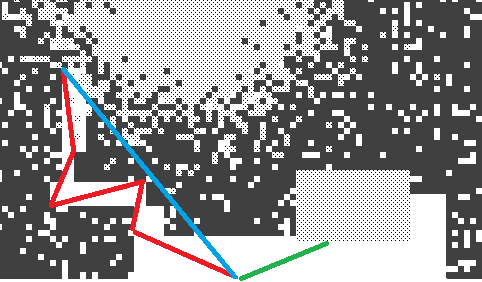
\includegraphics[width=0.75\textwidth]{chapters/chapter6/figures/problem-scalability-desertant.png}
\caption{Illustration of the inefficiencies of the desert ant algorithm's site fidelity in dense environments. Solid areas are non-prioritized items, white areas are free cells, and shaded areas are prioritized items. The red path is a hypothetical random walk performed by a robot, the blue path is the PI vector for the red random walk, and the green path is an alternative random walk.}
\label{fig:desertantsitefidelity}
\end{figure}

The honey bee algorithm uses site fidelity, and also communicates those sites to others. Despite the use of site fidelity mechanism similar to the desert ant algorithm, the honey bee algorithm is the most scalable. The reason why the site fidelity of the honey bee algorithm does not impact the scalability can be attributed the ability of the honey bee algorithm to adapt the swarm specialization ratio, $\tau$, to focus on foraging dense areas of obstacles, rather than having to expensively navigate around the obstacles. The ability of the honey bee algorithm to concentrate on clearing obstacles in highly dense environments will increase overall ease of access to the high quality sites, as discovered in Section~\ref{results:flexibility:environmentdistribution}. Thus efficiency of the honey bee algorithm in highly dense environments is improved. Therefore, the honey bee algorithm is the most scalable in terms of the problem size and complexity.

\begin{table}[]
\centering
\caption{Problem scalability for each environment density, $p$, for each algorithm}
\label{table:problemscalability}
\begin{tabular}{@{}llllll@{}}
\toprule
\textbf{$p$}                  & \textbf{0.05} & \textbf{0.2        } & \textbf{0.5}         & \textbf{0.7}         & \textbf{0.9}         \\ \midrule
\textbf{desert ant}           & 1    & 0.487816741 & 0.231581619 & 0.181686679 & 0.167953071 \\
\textbf{honey bee}            & 1    & 0.602283728 & 0.283264856 & 0.216749784 & 0.195686487 \\
\textbf{na\"ive}              & 1    & 0.501722909 & 0.256758663 & 0.195206738 & 0.174522486 \\
\textbf{Expected} & 1    & 0.25        & 0.1         & 0.071428571 & 0.055555556 \\ \bottomrule
\end{tabular}
\end{table}

\begin{figure}[!htb]
\centering
\resizebox{\textwidth}{!}{% GNUPLOT: LaTeX picture with Postscript
\begingroup
  \makeatletter
  \providecommand\color[2][]{%
    \GenericError{(gnuplot) \space\space\space\@spaces}{%
      Package color not loaded in conjunction with
      terminal option `colourtext'%
    }{See the gnuplot documentation for explanation.%
    }{Either use 'blacktext' in gnuplot or load the package
      color.sty in LaTeX.}%
    \renewcommand\color[2][]{}%
  }%
  \providecommand\includegraphics[2][]{%
    \GenericError{(gnuplot) \space\space\space\@spaces}{%
      Package graphicx or graphics not loaded%
    }{See the gnuplot documentation for explanation.%
    }{The gnuplot epslatex terminal needs graphicx.sty or graphics.sty.}%
    \renewcommand\includegraphics[2][]{}%
  }%
  \providecommand\rotatebox[2]{#2}%
  \@ifundefined{ifGPcolor}{%
    \newif\ifGPcolor
    \GPcolorfalse
  }{}%
  \@ifundefined{ifGPblacktext}{%
    \newif\ifGPblacktext
    \GPblacktexttrue
  }{}%
  % define a \g@addto@macro without @ in the name:
  \let\gplgaddtomacro\g@addto@macro
  % define empty templates for all commands taking text:
  \gdef\gplbacktext{}%
  \gdef\gplfronttext{}%
  \makeatother
  \ifGPblacktext
    % no textcolor at all
    \def\colorrgb#1{}%
    \def\colorgray#1{}%
  \else
    % gray or color?
    \ifGPcolor
      \def\colorrgb#1{\color[rgb]{#1}}%
      \def\colorgray#1{\color[gray]{#1}}%
      \expandafter\def\csname LTw\endcsname{\color{white}}%
      \expandafter\def\csname LTb\endcsname{\color{black}}%
      \expandafter\def\csname LTa\endcsname{\color{black}}%
      \expandafter\def\csname LT0\endcsname{\color[rgb]{1,0,0}}%
      \expandafter\def\csname LT1\endcsname{\color[rgb]{0,1,0}}%
      \expandafter\def\csname LT2\endcsname{\color[rgb]{0,0,1}}%
      \expandafter\def\csname LT3\endcsname{\color[rgb]{1,0,1}}%
      \expandafter\def\csname LT4\endcsname{\color[rgb]{0,1,1}}%
      \expandafter\def\csname LT5\endcsname{\color[rgb]{1,1,0}}%
      \expandafter\def\csname LT6\endcsname{\color[rgb]{0,0,0}}%
      \expandafter\def\csname LT7\endcsname{\color[rgb]{1,0.3,0}}%
      \expandafter\def\csname LT8\endcsname{\color[rgb]{0.5,0.5,0.5}}%
    \else
      % gray
      \def\colorrgb#1{\color{black}}%
      \def\colorgray#1{\color[gray]{#1}}%
      \expandafter\def\csname LTw\endcsname{\color{white}}%
      \expandafter\def\csname LTb\endcsname{\color{black}}%
      \expandafter\def\csname LTa\endcsname{\color{black}}%
      \expandafter\def\csname LT0\endcsname{\color{black}}%
      \expandafter\def\csname LT1\endcsname{\color{black}}%
      \expandafter\def\csname LT2\endcsname{\color{black}}%
      \expandafter\def\csname LT3\endcsname{\color{black}}%
      \expandafter\def\csname LT4\endcsname{\color{black}}%
      \expandafter\def\csname LT5\endcsname{\color{black}}%
      \expandafter\def\csname LT6\endcsname{\color{black}}%
      \expandafter\def\csname LT7\endcsname{\color{black}}%
      \expandafter\def\csname LT8\endcsname{\color{black}}%
    \fi
  \fi
    \setlength{\unitlength}{0.0500bp}%
    \ifx\gptboxheight\undefined%
      \newlength{\gptboxheight}%
      \newlength{\gptboxwidth}%
      \newsavebox{\gptboxtext}%
    \fi%
    \setlength{\fboxrule}{0.5pt}%
    \setlength{\fboxsep}{1pt}%
\begin{picture}(7200.00,5040.00)%
    \gplgaddtomacro\gplbacktext{%
      \csname LTb\endcsname%
      \put(740,640){\makebox(0,0)[r]{\strut{}$0$}}%
      \put(740,1020){\makebox(0,0)[r]{\strut{}$0.1$}}%
      \put(740,1400){\makebox(0,0)[r]{\strut{}$0.2$}}%
      \put(740,1780){\makebox(0,0)[r]{\strut{}$0.3$}}%
      \put(740,2160){\makebox(0,0)[r]{\strut{}$0.4$}}%
      \put(740,2540){\makebox(0,0)[r]{\strut{}$0.5$}}%
      \put(740,2919){\makebox(0,0)[r]{\strut{}$0.6$}}%
      \put(740,3299){\makebox(0,0)[r]{\strut{}$0.7$}}%
      \put(740,3679){\makebox(0,0)[r]{\strut{}$0.8$}}%
      \put(740,4059){\makebox(0,0)[r]{\strut{}$0.9$}}%
      \put(740,4439){\makebox(0,0)[r]{\strut{}$1$}}%
      \put(860,440){\makebox(0,0){\strut{}$0$}}%
      \put(1524,440){\makebox(0,0){\strut{}$0.1$}}%
      \put(2189,440){\makebox(0,0){\strut{}$0.2$}}%
      \put(2853,440){\makebox(0,0){\strut{}$0.3$}}%
      \put(3517,440){\makebox(0,0){\strut{}$0.4$}}%
      \put(4182,440){\makebox(0,0){\strut{}$0.5$}}%
      \put(4846,440){\makebox(0,0){\strut{}$0.6$}}%
      \put(5510,440){\makebox(0,0){\strut{}$0.7$}}%
      \put(6175,440){\makebox(0,0){\strut{}$0.8$}}%
      \put(6839,440){\makebox(0,0){\strut{}$0.9$}}%
    }%
    \gplgaddtomacro\gplfronttext{%
      \csname LTb\endcsname%
      \put(160,2539){\rotatebox{-270}{\makebox(0,0){\strut{}Problem Scalability ($PS$)}}}%
      \put(3849,140){\makebox(0,0){\strut{}Environment Density ($p$)}}%
      \put(3849,4739){\makebox(0,0){\strut{}Problem Scalability, $PS$, for each environment density $p$, for each algorithm}}%
      \put(5936,4276){\makebox(0,0)[r]{\strut{}Na\"ive}}%
      \put(5936,4076){\makebox(0,0)[r]{\strut{}Desert Ant}}%
      \put(5936,3876){\makebox(0,0)[r]{\strut{}Honey Bee}}%
      \put(5936,3676){\makebox(0,0)[r]{\strut{}Expected Scalability}}%
    }%
    \gplbacktext
    \put(0,0){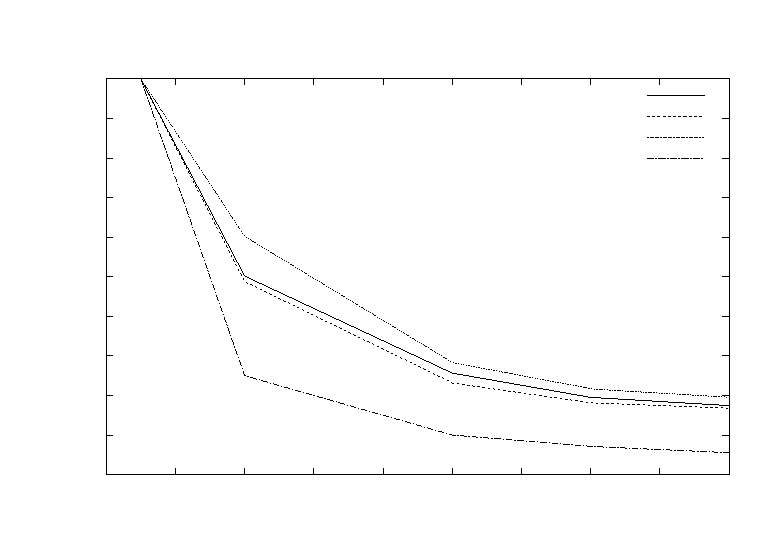
\includegraphics{chapters/chapter6/graphs/scalability/problemscalability}}%
    \gplfronttext
  \end{picture}%
\endgroup
}
\caption{Problem Scalability, $PS$, for each environment density $p$, for each algorithm}
\label{fig:problemscalability}
\end{figure}

\section{Robustness}
\label{results:robustness}
% describe fault tolerance, and provide rational arguments as to why it would be more or less 
As discussed in Section~\ref{robustness}, robot swarms achieve robustness by exhibiting the properties of redundancy, multiplicity of sensing and decentralized coordination. This study does not perform an empirical robustness study to specifically address how fault tolerant each algorithm is. Instead, this section provides rational arguments supported by empirical evidence to discuss each algorithm's robustness. Section~\ref{results:redundancy} discusses robustness in terms of the resulting redundancy of the swarms running each algorithm , and Section~\ref{results:decentralizedcoordination} discusses robustness in terms of decentralized coordination.

\subsection{Redundancy}
\label{results:redundancy}

As discussed in Section~\ref{robustness}, redundancy in a swarm is achieved by by giving all, or a portion of the robots in the swarm the same capabilities. In this way, if a percentage of the swarm malfunctions, the other robots have the capability to take the malfunctioning robots' place. A swarm demonstrates the highest level of redundancy when any robot can take on the role of any other robot that malfunctions in a swarm. 

For each of our experiments, each swarm is configured with an initial swarm specialization ratio (as discussed in Chapter~\ref{chap:experiment}) to enable a portion of robots to forage prioritized items and the another portion to forage non-prioritized items. 

If a portion of robots in a swarm malfunction or are destroyed, then the swarm specialization ratio will be affected. As shown in Section~\ref{results:flexibility}, the foraging efficiency of the na\"ive and desert ant algorithms were effected by the initial swarm specialization ratio $\tau$. It follows that if the swarm specialization ratio is unexpectedly changed during the swarm experiment, a change in the foraging efficiency of the swarm would persist for the experiment. In particular, consider the following extreme scenarios: 

Suppose all the robots which were foraging for prioritized items (for some $\tau > 0$) are destroyed or malfunction (thus $\tau=0$). Foraging efficiency would drop to 0, because no robots exist to forage prioritized items. Similarly, consider an environment where all prioritized items are blocked by non-prioritized items and that $\tau < 1$ . If all non-prioritized robots suffer a malfunction or are destroyed, then $\tau=1$ and no robots will be available to forage non-prioritized items. Foraging efficiency, $E_P$, will then drop to 0. 

As shown in Section~\ref{results:flexibility}, the honey bee algorithm experiences little change to efficiency when $\tau(0)$ is varied. The honey bee algorithm adapts the swarm specialization ratio, $\tau$, over time. It follows that, for the above scenarios, the honey bee algorithm will be able to re-adapt the swarm specialization ratio in order to replenish the robots that were destroyed. 

The robots controlled by the honey bee algorithm are homogeneous, in that every robot in the swarm has the ability to take on any of the roles required for the algorithm to function ( i.e. scout, unemployed forager, employed forager), as well as to adapt to forage either prioritized or non-prioritized items. It follows that the swarms running the honey bee algorithm are more redundant than swarms running the the desert ant algorithm and the na\"ive algorithm.

\subsection{Decentralized Coordination}
\label{results:decentralizedcoordination}

Decentralized coordination can be attained by creating algorithms that do not depend on decisions, actions or sensor readings of any single individual or a few individuals of the swarm. 

The robots of the desert ant and na\"ive algorithm do not depend on each other and there is no centralized coordination. Despite no explicit coordination mechanism between individuals, robots coordinate implicitly by using obstacles avoidance to avoid obstructing each other. In that way, the robots in the swarm avoid hitting each other. The mechanism for obstacle avoidance is entirely decentralized, because each robot only depends on it's own internal sensors. All other operations of the robots in the desert and and na\"ive algorithm are decentralized as they do not depend on any other individual.

On the other hand, the honey bee algorithm uses communication as a coordination mechanism in order to recruit foragers to areas with a high density of prioritized items, as described in Section~\ref{honeybeeforaging}. If the scout robots experience a fault in evaluating the quality of a site (for example, detecting that a site is of high quality when it is actually a site of poor quality), then foragers will be incorrectly recruited to forage sites of low quality. Only a few individuals (the scouts) can coordinate the swarm and therefore any faults in the scout robots, may negatively influence effect the efficiency of the entire swarm. The coordination mechanism of the honey bee algorithm is not entirely decentralized.


To provide further evidence that the scout robots can mislead the swarm to incorrectly foraging areas that have low quality resources, an examination of the average time spent, per item foraged, per robot, in the recruitment state is provided as follows: 

Table~\ref{averagetimerecruitment} and Figure~\ref{fig:recruitmenttime} illustrate the average timesteps spent performing recruitment, $t_{recruitment}$, per robot, per (both prioritized and non-prioritized) item foraged, for the honey bee algorithm, for each environment distribution. The results were averaged over each environment item type ratio, $r$. 

\begin{table}[]
\centering
\caption{Average time steps, per robot, per prioritized item foraged, that were spent performing recruitment for the honey bee algorithm, in each environment distribution, for each environment item type ratio $r$.}
\label{averagetimerecruitment}
\begin{tabular}{@{}lllll@{}}
\toprule
$r$            & \textbf{clustered} & \textbf{gaussian} & \textbf{uniform} & \textbf{vein} \\ \midrule
\textbf{0}        & 0        & 0       & 0      & 0   \\
\textbf{0.2}      & 0.119486333        & 0.152139262       & 0.11962912       & 0.160737113   \\
\textbf{0.25}     & 0.126752914        & 0.144484389       & 0.127568794      & 0.158813789   \\
\textbf{0.333333} & 0.140492087        & 0.135243974       & 0.139460537      & 0.151803907   \\
\textbf{0.5}      & 0.161644793        & 0.15738657        & 0.16335568       & 0.168543223   \\
\textbf{0.666667} & 0.181659692        & 0.174940591       & 0.183477822      & 0.151701447   \\
\textbf{0.75}     & 0.179285021        & 0.177420259       & 0.183721153      & 0.171862739   \\
\textbf{0.8}      & 0.182807781        & 0.182650316       & 0.186144899      & 0.190969001   \\
\textbf{1}        & 0.167397088        & 0.172990294       & 0.163048904      & 0.219223401   \\ \bottomrule
\end{tabular}
\end{table}


\begin{figure}[!htb]
\centering
\resizebox{\textwidth}{!}{% GNUPLOT: LaTeX picture with Postscript
\begingroup
  \makeatletter
  \providecommand\color[2][]{%
    \GenericError{(gnuplot) \space\space\space\@spaces}{%
      Package color not loaded in conjunction with
      terminal option `colourtext'%
    }{See the gnuplot documentation for explanation.%
    }{Either use 'blacktext' in gnuplot or load the package
      color.sty in LaTeX.}%
    \renewcommand\color[2][]{}%
  }%
  \providecommand\includegraphics[2][]{%
    \GenericError{(gnuplot) \space\space\space\@spaces}{%
      Package graphicx or graphics not loaded%
    }{See the gnuplot documentation for explanation.%
    }{The gnuplot epslatex terminal needs graphicx.sty or graphics.sty.}%
    \renewcommand\includegraphics[2][]{}%
  }%
  \providecommand\rotatebox[2]{#2}%
  \@ifundefined{ifGPcolor}{%
    \newif\ifGPcolor
    \GPcolorfalse
  }{}%
  \@ifundefined{ifGPblacktext}{%
    \newif\ifGPblacktext
    \GPblacktexttrue
  }{}%
  % define a \g@addto@macro without @ in the name:
  \let\gplgaddtomacro\g@addto@macro
  % define empty templates for all commands taking text:
  \gdef\gplbacktext{}%
  \gdef\gplfronttext{}%
  \makeatother
  \ifGPblacktext
    % no textcolor at all
    \def\colorrgb#1{}%
    \def\colorgray#1{}%
  \else
    % gray or color?
    \ifGPcolor
      \def\colorrgb#1{\color[rgb]{#1}}%
      \def\colorgray#1{\color[gray]{#1}}%
      \expandafter\def\csname LTw\endcsname{\color{white}}%
      \expandafter\def\csname LTb\endcsname{\color{black}}%
      \expandafter\def\csname LTa\endcsname{\color{black}}%
      \expandafter\def\csname LT0\endcsname{\color[rgb]{1,0,0}}%
      \expandafter\def\csname LT1\endcsname{\color[rgb]{0,1,0}}%
      \expandafter\def\csname LT2\endcsname{\color[rgb]{0,0,1}}%
      \expandafter\def\csname LT3\endcsname{\color[rgb]{1,0,1}}%
      \expandafter\def\csname LT4\endcsname{\color[rgb]{0,1,1}}%
      \expandafter\def\csname LT5\endcsname{\color[rgb]{1,1,0}}%
      \expandafter\def\csname LT6\endcsname{\color[rgb]{0,0,0}}%
      \expandafter\def\csname LT7\endcsname{\color[rgb]{1,0.3,0}}%
      \expandafter\def\csname LT8\endcsname{\color[rgb]{0.5,0.5,0.5}}%
    \else
      % gray
      \def\colorrgb#1{\color{black}}%
      \def\colorgray#1{\color[gray]{#1}}%
      \expandafter\def\csname LTw\endcsname{\color{white}}%
      \expandafter\def\csname LTb\endcsname{\color{black}}%
      \expandafter\def\csname LTa\endcsname{\color{black}}%
      \expandafter\def\csname LT0\endcsname{\color{black}}%
      \expandafter\def\csname LT1\endcsname{\color{black}}%
      \expandafter\def\csname LT2\endcsname{\color{black}}%
      \expandafter\def\csname LT3\endcsname{\color{black}}%
      \expandafter\def\csname LT4\endcsname{\color{black}}%
      \expandafter\def\csname LT5\endcsname{\color{black}}%
      \expandafter\def\csname LT6\endcsname{\color{black}}%
      \expandafter\def\csname LT7\endcsname{\color{black}}%
      \expandafter\def\csname LT8\endcsname{\color{black}}%
    \fi
  \fi
    \setlength{\unitlength}{0.0500bp}%
    \ifx\gptboxheight\undefined%
      \newlength{\gptboxheight}%
      \newlength{\gptboxwidth}%
      \newsavebox{\gptboxtext}%
    \fi%
    \setlength{\fboxrule}{0.5pt}%
    \setlength{\fboxsep}{1pt}%
\begin{picture}(7200.00,5040.00)%
    \gplgaddtomacro\gplbacktext{%
      \csname LTb\endcsname%
      \put(860,640){\makebox(0,0)[r]{\strut{}$0$}}%
      \put(860,1472){\makebox(0,0)[r]{\strut{}$0.05$}}%
      \put(860,2304){\makebox(0,0)[r]{\strut{}$0.1$}}%
      \put(860,3135){\makebox(0,0)[r]{\strut{}$0.15$}}%
      \put(860,3967){\makebox(0,0)[r]{\strut{}$0.2$}}%
      \put(860,4799){\makebox(0,0)[r]{\strut{}$0.25$}}%
      \put(980,440){\makebox(0,0){\strut{}$0$}}%
      \put(2152,440){\makebox(0,0){\strut{}$0.2$}}%
      \put(3324,440){\makebox(0,0){\strut{}$0.4$}}%
      \put(4495,440){\makebox(0,0){\strut{}$0.6$}}%
      \put(5667,440){\makebox(0,0){\strut{}$0.8$}}%
      \put(6839,440){\makebox(0,0){\strut{}$1$}}%
    }%
    \gplgaddtomacro\gplfronttext{%
      \csname LTb\endcsname%
      \put(160,2719){\rotatebox{-270}{\makebox(0,0){\strut{}$t_{recruitment}$}}}%
      \put(3909,140){\makebox(0,0){\strut{}Environment item type ratio ($r$)}}%
      \put(5936,4636){\makebox(0,0)[r]{\strut{}clustered}}%
      \put(5936,4436){\makebox(0,0)[r]{\strut{}gaussian}}%
      \put(5936,4236){\makebox(0,0)[r]{\strut{}uniform}}%
      \put(5936,4036){\makebox(0,0)[r]{\strut{}vein}}%
    }%
    \gplbacktext
    \put(0,0){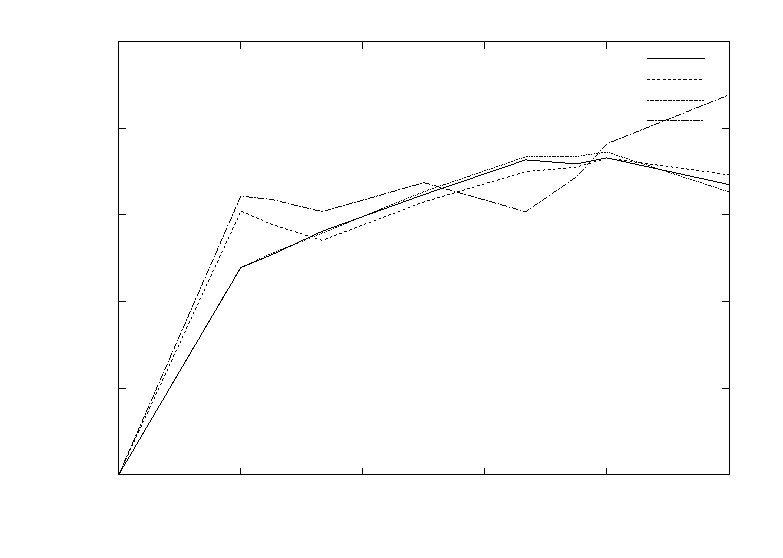
\includegraphics{chapters/chapter6/graphs/robustness/robustness-recruitment-type-honeybee}}%
    \gplfronttext
  \end{picture}%
\endgroup
}
\caption{Average timesteps spent performing recruitment activities by robots of the swarm for each item foraged, $t_{recruitment}$, for the honey bee algorithm, per item distribution, for each environment item type ratio, $r$.}
\label{fig:recruitmenttime}
\end{figure}

Table~\ref{averagetimerecruitment} illustrate that on average each robot spent at least 11.96\% of it's the total foraging time recruiting other robots to forage higher quality areas, for all values of $r > 0$. This is particularly relevant for uniformly distributed environments, with a low ratio of prioritized items ($r = 0.2$), because it is unlikely that sites of high quality do not exist, because the prioritized items will be scarce and scattered. Table~\ref{averagetimerecruitment} shows that average each robot spent at least 11.96\% of it's the total foraging time recruiting other robots to forage higher quality areas, that don't exist. This means that the scouts were recruiting other robots to forage areas that were not of a high quality. The fact that scouts can mislead the swarm to foraging sites with low quality, shows that the honey bee algorithm is less robust.

Figure~\ref{fig:recruitmenttime} also demonstrates that recruitment occurs more regularly for gaussian and vein environments, which means that the honey bee algorithm performs more recruitment in environments which exhibit high quality sites.

\section{Summary}
\label{results:summary}

This chapter presented the results of the experiments and performed analysis of the major properties of swarm robotics, for each algorithm. The results were discussed around four axes: efficiency, flexibility, robustness and scalability. 

Section~\ref{results:efficiency} presented an overview of foraging efficiency of each algorithm. The results showed that the honey bee algorithm was the most efficient over all environments and swarm configurations, while the desert ant was the next most efficient and the na\"ive algorithm was the least efficient.

Section~\ref{results:flexibility} analysed the flexibility of each algorithm. Flexibility was analysed in terms of flexibility over environments prioritized item ratio, $F_r$, and flexibility over environment distribution type, $F_{ED}$. 

Section~\ref{results:prioritizeditemratio} concluded that the honey bee algorithm was the most flexible in terms of prioritized item ratio. It was shown that the honey bee algorithm's flexibility is a result of honey bee algorithm's ability to adapt the specialization ratio $\tau$, via the honey bee algorithm's division of labour mechanism. The division of labour mechanism allowed the honey bee robots to more efficiently forage an environment for any given environment item ratio $r$. The na\"ive algorithm was more flexible than the desert ant algorithm, in terms of environment item distribution. The na\"ive algorithm's perceived flexibility is attributed to the fact that the na\"ive algorithm suffers far lower efficiency across all environment item ratios, suggesting that it appears flexible since it performs equally bad across all values of $r$, unable to exploit any differences between the environments. 

Section~\ref{results:flexibility:environmentdistribution} concluded that the honey bee algorithm is the most flexible, in terms of environmental distribution, followed by the desert ant algorithm and lastly the na\"ive algorithm. The honey bee algorithm was determined to be more flexible, due to it's ability to adapt the specialization ratio to better suit the types of items that are reachable by the swarm. The adaptation of specialization ratio allowed the honey bee swarm to focus on foraging non-prioritized when only non-prioritized items were reachable, and then adjust the ratio to focus on foraging prioritized items when prioritized items were reachable. The desert ant and na\"ive algorithms, without the ability to adjust $\tau$ to more effectively forage the ratio of reachable objects, are less flexible than the honey bee algorithm.
  The na\"ive algorithm's perceived flexibility over environment distribution, compared to the desert ant algorithm, was attributed to the same reasons as determined by Section~\ref{results:prioritizeditemratio}. 
  
Section~\ref{results:scalability} evaluated scalability in terms of swarm scalability, $SS$ and $PS$. Section~\ref{results:swarmscalability} determined that the scalability of all algorithms, in terms of swarm scalability, was sub-linear. More specifically, the na\"ive algorithm was the most scalable in terms of swarm density, and then the desert ant and honey bee algorithms which exhibited similar scalability. The desert ant algorithm's poor performance, compared to the na\"ive algorithm was attributed the desert ant algorithm's use of site fidelity. A rational argument was presented that argued the desert ant algorithm's site fidelity increased inter-robot interference, which resulted in poor efficiency when swarm density was high. The honey bee algorithm was shown to be slightly more scalable than the desert ant algorithm, due to the honey bee algorithm's attempt to regulate the number of active foragers by division of labour. The difference in swarm scalability between the desert ant algorithm and the honey bee algorithm was very small, suggesting that the regulation of active foragers was not functioning very well. The honey bee algorithm's ability to regulate the number of active foragers as swarm densities increase, was shown to be ineffective. 

Section~\ref{results:problemscalability} determined that the honey bee algorithm is the most scalable in terms of problem scalability, followed by the na\"ive algorithm, and lastly the desert ant algorithm. The discussion showed that the desert ant's performed comparatively worse than the na\"ive algorithm in terms of problem scalability, due to the desert ant algorithm's use of site fidelity to exploit good search areas. The section determined the na\"ive algorithm's ability to explore more than the desert ant algorithm, resulted in better problem scalability. The honey bee algorithm was the most scalable in terms of problem scalability. The problem scalability of the honey bee algorithm can be attributed to the ability of the honey bee algorithm to adapt $\tau$ to help clear non-prioritized items, which resulted in lower inter-robot and environmental interference.

Section~\ref{results:robustness} addressed robustness of each of the algorithms, in terms of redundancy and decentralized coordination. Section \ref{results:redundancy} showed that the honey bee algorithm has the highest redundancy, since the swarm is homogeneous. The honey bee swarm is homogeneous as the robots can switch specialization, rather than being set to forage only a specific item type. The desert ant algorithm and na\"ive algorithm robots can only forage a single item type, which is pre-configured and thus their swarms are heterogeneous, and thus the swarms are less redundant.

Section~\ref{results:decentralizedcoordination} determined that the desert ant and na\"ive algorithm are the most robust in terms of decentralized coordination, since neither algorithm employ a coordination mechanism between robots of the swarm. The honey bee algorithm was determined to be the least robust in terms of decentralized coordination. The honey bee algorithm's coordination mechanism was sensitive to faults in certain individuals where invalid information was communicated to the swarm and the invalid information impacted efficiency.

%DONT THINK THIS GOES HERE%
Taking the discussion of the flexibility, scalability, and robustness of each algorithm back to foraging efficiency: The honey bee algorithm exhibited a high level of flexibility, problem scalability, and redundancy, resulting in greater overall efficiency than the desert ant algorithm and na\"ive algorithm. On the other hand, despite the na\"ive algorithm exhibiting better scalability than the desert ant algorithm, the desert ants algorithm's ability to exploit high quality areas, resulted in greater average performance than the na\"ive algorithm.

%%%%%%%%%%%%%%%%%%%%%%%%%%%%%%%%%%%%%%%%%%%%%%%%%
%%%%%%%%%%%%%%%%%%%%%%%%%%%%%%%%%%%%%%%%%%1%%%%%%%
